\documentclass[12pt]{exam}
\usepackage{graphicx} % Required for inserting images
\usepackage{mathtools}
\usepackage{amsmath}
\usepackage{amssymb}
\usepackage[
backend=bibtex,
style=ieee,
]{biblatex}
\usepackage{hyperref}
\usepackage{float}
\usepackage{appendix}
\usepackage{subcaption}
\usepackage[table]{xcolor}
\usepackage{array}
\usepackage{setspace}
\usepackage[left=1in,right=1in,top=1in,bottom=1in]{geometry}
\usepackage{xcolor}
\usepackage{listings}
\usepackage{minted}

\lstset{
  language=R,
  basicstyle=\ttfamily\small,
  keywordstyle=\color{blue},
  commentstyle=\color{gray},
  stringstyle=\color{green!60!black},
  numbers=left,
  numberstyle=\tiny,
  breaklines=true,
  frame=single
}



\addbibresource{report_sources.bib}
\addbibresource{proposal_sources.bib}
\renewcommand{\contentsname}{Table of Contents} % Sets title of TOC

\newcommand{\onesidedhyp}[1]{
\begin{matrix}
H_0 &: #1 \le 0 \\
H_a &: #1 > 0
\end{matrix}
}

\begin{document}
\setlength{\parindent}{0pt}

\begin{titlepage}
    \begin{center}
        \vspace*{1cm}

        {\huge \textbf{The impact of of gain-based versus loss-based feedback on mental math accuracy and response times}}

        \vspace*{1.5cm}

        \textbf{Gabriella Wang, Mahtasim Bhuiyan, Rahi Thurairajah}
        
        \textit{MIE286H1S (Probability and Statistics) Research Project}
        \vspace*{0.5cm}

        Division of Engineering Science, University of Toronto
        \vspace*{0.5cm}
        
        April 7 2026
        \vspace*{0.5cm}
\hrule
\end{center}
\end{titlepage}
\newpage
\tableofcontents
\newpage
\setcounter{page}{1}  % so title page and TOC aren't numbered

\section{Introduction and Background}
A common method of assigning a score to someone’s performance on a task is to assign them points for successfully completing parts of the task. There are two main ways these points are assigned. The first is gain-based; someone begins at 0 points and slowly earns points until they complete the task. One such example is in education; on an exam, students begin with 0 points – as the exam is marked, they earn points for each correct question, until the end of the exam, at which point they have a final score (e.g., a student may gain 20 points for answering question 1 of an exam correctly; at the end, they may have 75/100 points, with 25 points not earned for incorrect work). The second type is loss-based, with someone starting with a maximum number of points and slowly losing points until they complete the task or lose all their points. This is common in video games, with the points being “lives”.\newline

The goal of this study was to see which of these two forms of feedback resulted in higher performance on mental math tests (or if there was no measurable difference). Humans often assign value to things that they “own” (i.e., the points), even if they have no intrinsic value; as a result, we hypothesized that the loss-based feedback would result in higher average scores on the tests as participants would be motivated to keep their points. By contrast, with the gain-based feedback, participants do not lose anything for getting a question wrong, potentially reducing the perceived cost of failure. This is consistent with Prospect Theory \cite{prospect-theory}, which suggests humans weigh losses more heavily than gains, potentially leading to stronger behavioural responses under loss-based conditions.\newline

Existing research from the NIH supports this \cite{nih-paper}, suggesting that people are more sensitive to losses than equivalent gains (i.e., losing 1 point feels more negative than earning 1 point feels positive). A study published in the Economics of Education Review \cite{econeducationrev} found that in a multiple-choice vocabulary exam, the “loss frame” of losing points from a starting “endowment” for incorrect answers drove increased effort and overall performance as opposed to the “gain frame” of starting from 0 and earning points for correct answers. Accordingly, this study aimed to test whether this perceived difference would translate to actual differences in task performance. Specifically, it investigates the question:

\begin{center}
    \textit{Does loss-based feedback significantly affect accuracy and response time in time-constrained mental math tasks when compared to gain-based feedback?}
\end{center}

\section{Methods}
\subsection{Experimental Process}
The experiment followed a mixed design (between-subjects for feedback type and within-subject for baseline vs feedback), with participants (family members and fellow students) either completing a loss-based set of questions, or a gain-based set of questions. All participants also completed a baseline test with no feedback before the feedback-based set. Both sets had 20 multiple-choice, 2-to-3-digit arithmetic questions, each with 3 answer choices with a time limit of 10 seconds per question to ensure that participants did not spend lots of time on each question (which would have resulted in all participants getting 20/20, making accuracy measurements effectively pointless). We administered the questions to each participant on a laptop through a window in the center of the screen created using the Python library Pygame \cite{pygame}. 

During the baseline trials, upon clicking an answer (or the countdown for the question hitting 0 without an answer selected), the correctness of the user’s selection was not indicated, and the display immediately moved on to the next question (see Figure \ref{fig:baseline-test}). 
During the gain-based trials, there was a “Points” counter in the top right which started at 0 and increased by 1 for every correctly answered question but did not change for any incorrectly answered or unanswered question (see Figure \ref{fig:gain-test}). 
During the loss-based trials, the same “Points” counter instead started at 20 and decreased by 1 for every incorrectly answered or not answered questions but did not change for any correctly answered questions (see Figure \ref{fig:loss-test}).

\begin{figure}[H]
    \centering
    \begin{subfigure}{0.45\textwidth}
    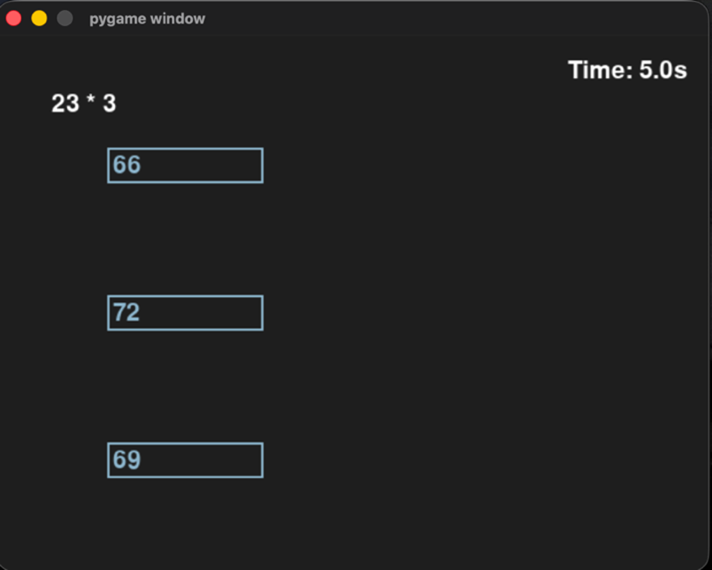
\includegraphics[width=\textwidth]{images/baseline.png}
        \caption{A screenshot of a baseline trial featuring no feedback on the user’s selections or total score and simply advancing after an answer}
        \label{fig:baseline-test}
    \end{subfigure}
    \hfill
    \begin{subfigure}{0.45\textwidth}
        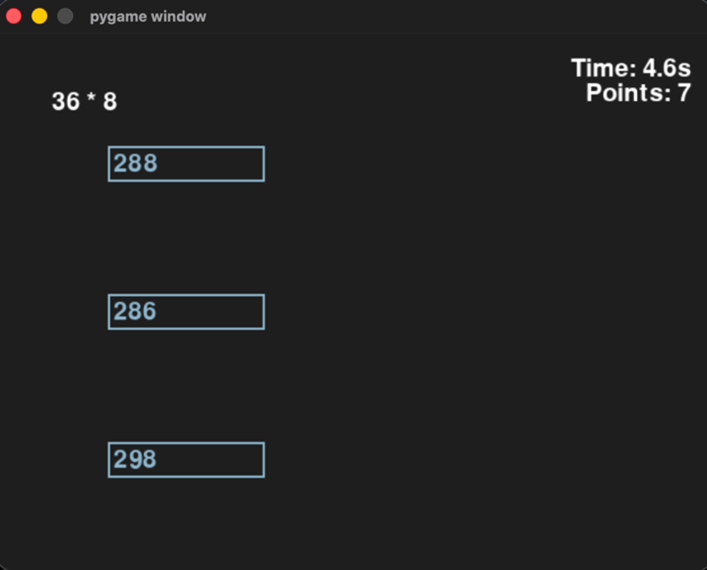
\includegraphics[width=\textwidth]{images/gain.png}
        \caption{A screenshot of a gain-based trial featuring a point counter starting from 0 which increased by 1 for each correct selection}
        \label{fig:gain-test}
    \end{subfigure}
    \begin{subfigure}{0.45\textwidth}
        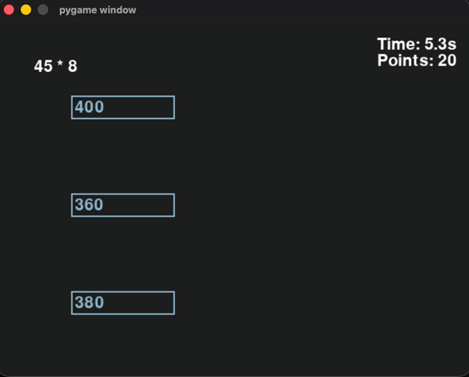
\includegraphics[width=\textwidth]{images/loss.png}
        \caption{A screenshot of a loss-based trial featuring a point counter starting from 20 which decreased by 1 for each incorrect selection}
        \label{fig:loss-test}
    \end{subfigure}
    \caption{The three different feedback conditions}
    \label{fig:test-program}

\end{figure}

\subsection{Variables}

The dependent variables in this experiment are accuracy, measured as the proportion of correct questions out of 20, and response time in milliseconds (i.e., time taken from the question appearing to the participant clicking an answer).
The independent variable is the type of feedback the participant receives (either gain-based or loss-based). Participants were randomly assigned to one of these groups through a coin flip to prevent bias.\newline

Baseline performance was treated as a covariate to account for inherent differences in participant ability. Since participants may differ in their natural mental math skill, comparing only raw performance between groups could confound the effect of feedback type with individual ability. By analyzing the change in performance relative to baseline (i.e., $\Delta a$ and $\Delta \tau$), we can isolate the effect of the feedback condition more effectively.

\subsection{Control Conditions}
We conducted all the trials in as quiet of an environment as was feasible to minimize any external noise distracting the participants from the tasks. We were careful to look and step away from the participant as soon as each trial began to avoid adding any emotional pressure on participants from being watched. All participants received the same set of questions (one set for the baseline and another set which was the same for feedback conditions) rather than giving each participant unique questions, to ensure that everyone had an equally difficult set of questions. Before each experiment, a standard script was read to the participant with no additions or deviations to reduce variability between trials. Participants in the gain-based test were not told how many questions were in the test, to prevent the possibility of loss-based thinking triggered by interpreting their points as a fraction of the total possible perfect score (i.e. 15/20 points, versus 15 points). For consistency, those in the loss-based test were not told this either.

\subsection{Limitations}
While the gain-based and loss-based conditions used identical question sets, the baseline set differed from the feedback set, so it is possible that participants found one harder than the other due to the questions alone. This may have affected the trial accuracy and response time results and limits fairness of comparisons between baseline and feedback results. Additionally, the trials were not conducted in perfect silence, and not all in the same room, so it is possible external noise affected participants’ concentration to varying degrees. 
Finally, the participants were limited to our peers and family members. Given that our peers are in Engineering Science, they likely have stronger-than-average math skills and so are not a representative sample.

\section{Analysis}
\subsection{Hypotheses}

This study predicts that loss-based feedback results in higher accuracy ($a$) on mental math questions and longer response times ($\tau$). Research by the NIH \cite{nih-paper} suggests that both loss-based and gain-based feedback result in better performance on tasks that require fast-responses, such as this study’s mental math problems. Thus, this study also hypothesizes that both forms of feedback will result in higher accuracy, though it is important to note that the difficulty of the feedback and baseline problem sets may be different, which can limit the fairness of the comparison. However, this research also found that tasks that require effort tend to be performed better with loss-based feedback as participants put more effort into their responses. Mental math requires cognitive effort, suggesting that loss-based feedback would result in higher accuracy on mental math questions, and due to increased effort, longer response times.\newline

One-tailed $t$-tests were conducted to test the hypotheses described above given that they suggest differences in population means strictly above 0. These hypotheses were formulated based on literature, as mentioned in the introduction.\cite{prospect-theory}

To compare the accuracy and response times of tests with loss-based feedback and gain-based feedback, tests were conducted both comparing the means of these samples, as well as comparing the means of the differences in accuracy and response time between the feedback tests and the baseline tests (called the relative accuracy $\Delta a$  and response time $\Delta\tau$ , respectively) to account for differences in skills between participants so that each participant effectively acts as their own control \footnote{An alternative approach would be to use an analysis of covariance (ANCOVA) to control for baseline performance. However, given the relatively small sample size and the simplicity of the experimental design, we chose to use difference scores instead}. For tests that indicate no significant difference, we conducted two-tailed $t$-tests to investigate whether there is any difference at all between the groups (though these should be treated as exploratory). All hypotheses are described in Table \ref{tab:hypotheses} below:

\begin{table}[H]
    \centering
    \caption{Null and alternative hypotheses for one-tailed, two-sample $t$-tests comparing the feedback conditions}
    \begin{tabular}{|c|p{6cm}|c|}
        \hline
        Hypothesis \# & Hypothesis Description & Hypothesis for One-tailed, Two-Sample $t$-test \\
        \hline
        1 & Loss-based feedback results in higher accuracy than gain-based feedback (NOT accounting for differences in skill level) & $\onesidedhyp{\mu_{a,L} - \mu_{a,G}}$ \\ 
        \hline
        2 & Loss-based feedback results in higher accuracy than gain-based feedback (accounting for differences in skill level) & $\onesidedhyp{\mu_{\Delta a,L} - \mu_{\Delta a,G}}$ \\ 
        \hline
        3 & Loss-based feedback results in higher response times than gain-based feedback (NOT accounting for differences in skill level) & $\onesidedhyp{\mu_{\tau,L} - \mu_{\tau,G}}$ \\ 
        \hline
        4 & Loss-based feedback results in higher response times than gain-based feedback (accounting for differences in skill level) & $\onesidedhyp{\mu_{\Delta \tau,L} - \mu_{\Delta \tau,G}}$\\ 
        \hline
        5 & Loss-based feedback results in higher accuracy than having no feedback & $\onesidedhyp{\mu_{a,L}-\mu_{a,baseline}}$\\ 
        \hline
        6 & Loss-based feedback results in higher response times than having no feedback & $\onesidedhyp{\mu_{\tau,L}-\mu_{\tau,baseline}}$\\ 
        \hline
        7 & Gain-based feedback results in higher accuracy than having no feedback & $\onesidedhyp{\mu_{a,G}-\mu_{a,baseline}}$\\ 
        \hline
    \end{tabular}
    \label{tab:hypotheses}
\end{table}

\subsection{Analysis Process}
To compute accuracy and response time, the mean accuracy and response time for each participant (across the 20 trials) was computed using:

\begin{equation}
    \label{eq:participant-accuracy}
    \bar{a}_{participant}=\frac{\text{\# of correct questions}}{20}
\end{equation}

\begin{equation}
    \label{eq:participant-response-time}
    \bar{\tau}_{participant} = \frac{1}{20} \sum_{i=1}^{20}\tau_i
\end{equation}

Where $\tau_i$ is the time taken to answer the $i$th question in ms. If a question was not answered within the 10 second time limit, it was treated as incorrect, with a response time of 10 000 ms (10 seconds). The sample mean and standard deviation were then calculated using these averaged accuracy and response times. The participants’ baseline performance can be treated as a covariate, which we account for by measuring the relative scores for both accuracy and response time (i.e., $\Delta a_{participant}= a_{feedback} - a_{baseline}$ and  $\Delta \tau_{participant}=\tau_{feedback}-\tau_{baseline}$ for each participant).\newline

The problem set program stored data in the form of JSON files. This data was then converted to R dataframes. Before we conducted the $t$-tests, we visualized the data using histograms and box plots to get an image of the distributions using basic R functions. This allowed us to identify differences between the distributions of datasets and identify skew. Q-Q plots were employed to determine whether data follows a normal distribution. We then conducted two-sample $t$-tests for the differences in means shown in Table \ref{tab:hypotheses} for unknown and unequal variance (known as Welch’s $t$-test). Using a 95\% confidence interval, the p-values of these tests were extracted to determine whether differences in mean associated with the above hypotheses were significant. A significance level of $\alpha = 0.05$ was used \cite{p-0.05}, corresponding to a 5\% risk of a Type I error \cite{lin2018bias} (incorrectly rejecting a true null hypothesis). Given the relatively small sample size, there is also an increased risk of Type II error, meaning that true effects may not be detected \cite{sample-size-effect}.

\section{Results}
\subsection{Box Plots and Histograms}
We computed the mean accuracy and response time from the JSON files for each participant and plotted this data on histograms (see Appendix \ref{appdx:histograms}). GIven the small sample size, it is difficult to draw any conclusions from the histograms, but most are relatively symmetrically distributed, with some showing skews. To properly compare the results between the two feedback types, we began by computing the sample mean and standard deviation for each group, giving us the results in Table \ref{tab:results-summary} below: 

\begin{table}[H]
    \centering
    \caption{Sample mean ($\bar{x}$) and standard deviation $S$ for accuracy ($a$) and response time in ms ($\tau$) for loss-based feedback, gain-based feedback, and baseline trials. "Baseline" refers to the no feedback condition grouped according to the subsequent feedback condition completed by the participants. $n_{loss}=14$ and $n_{gain} = 16$.}
    \begin{tabular}{|c|c|c|c|c|}
    \hline
         & Baseline (gain-based) & Baseline (loss-based) & Gain-Based & Loss-Based \\
    \hline
        $\bar{a}$ & 0.8406 & 0.8857 & 0.7219 & 0.7357\\
    \hline
        $S_{a}$ & 0.1417 & 0.1200 & 0.1505 & 0.1008 \\
    \hline
        $\bar{\tau}$ (ms) & 4048.6125 & 3997.6679 & 4104.0250 & 4104.2036 \\
    \hline
        $S_{\tau}$ (ms) & 1203.3657 & 765.1296 & 877.4196 & 830.3003 \\
    \hline
    \end{tabular}
    \label{tab:results-summary}
\end{table}

We can plot our data as a boxplot, seen below in Figure \ref{fig:boxplots}

\begin{figure}[H]
    \centering
    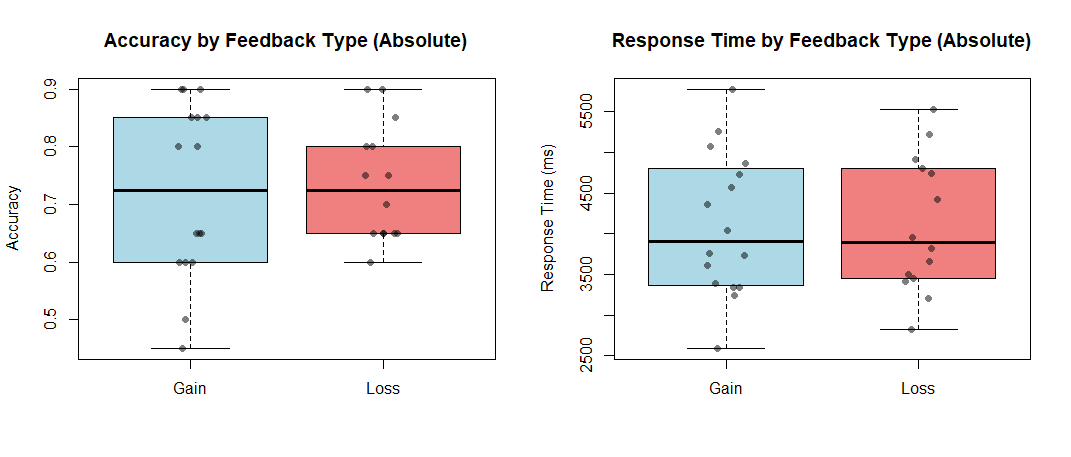
\includegraphics[width=1\linewidth]{images/boxplots of absolute accuracy and response times .png}
    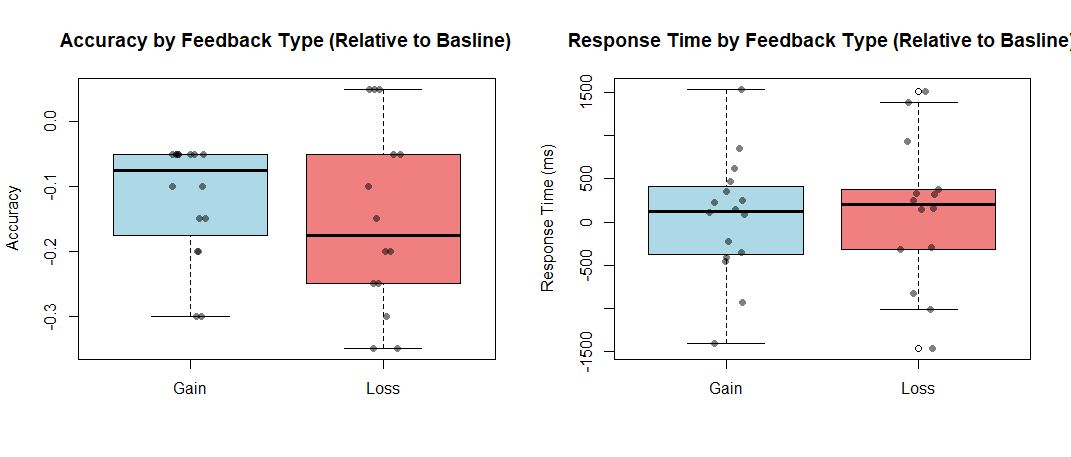
\includegraphics[width=1\linewidth]{images/boxplots of relative accuracy by feedback type.png}
    \caption{Boxplots for Accuracy and Response Time as absolute and relative scores. These can also be found in Appendix \ref{appdx:boxplots}}
    \label{fig:boxplots}
\end{figure}

From the boxplots we can see that the two groups have similar median accuracy and response times. The gain-based feedback shows a wider spread of data, though the accuracy shows some clustering at the upper end of the plot (suggesting there may be some outliers in that category). These visual patterns suggest that any differences between the groups are likely small; however, visual inspection alone is insufficient to determine statistical significance. We can confirm this more rigorously using $t$-tests.

\subsection{Q-Q plots}
Prior to using $t$-tests to test our hypothesis, we checked the assumptions of independence and normality. We did not assume equal variances. Independence between participants is satisfied due to the between-subjects assignment of feedback type. However, measurements within each participant (baseline vs. feedback) are dependent. We accounted for this by measuring the difference in scores. \newline

To check for normality, we created Q-Q plots with a 95\% confidence interval envelope for the accuracy and response time (both for absolute scores and scores relative to the baseline), which can be found in Appendix \ref{appdx:qq-plots}. These plots show that the response times are approximately normally distributed as the points lie relatively close to a straight line and all lie within the 95\% CI envelope. This is also the case for the loss-based accuracies. The gain-based accuracies (in particular the relative scores) show some deviation from normality with a flattening in the upper quantiles of the plot; however all but one of these points lie within the envelope. This suggests that many participants performed approximately the same on the baseline and gain-based tests, leading to limited variability among the higher relative scores. Given that nearly all data points lie along a straight line (within the tolerance of the 95\% CI) a normality assumption is still reasonable here, so applying $t$-tests here is reasonable.

\subsection{$t$-tests}

\begin{table}[H]
    \centering
    \caption{One-sided $t$-test results for accuracy and response times, comparing both raw and relative scores. The right endpoint of all confidence intervals is +$\infty$.}
    \begin{tabular}{|c|c|c|c|c|c|c|c|}
    \hline
        Test \# & 1 & 2 & 3 & 4 & 5 & 6 & 7\\ 
    \hline
        $p$-value & 0.3871 & 0.8286 & 0.5726 & 0.3435 & 0.9991 & 0.3233 & 1 \\
    \hline
        $t$-statistic & 0.2903 & -0.9714 & -0.1848 & 0.4077 & -3.8944 & 0.4693 & -5.3245 \\
    \hline
        95\% CI left endpoint & -0.0701 & -0.1189 & -628.1309 & -386.8565 & -0.2182 & -295.4922  & -0.1578 \\
    \hline
        $dof$ & 22.409  & 20.396 & 25.704 & 23.326 & 13 & 13 & 15\\
    \hline
    \end{tabular}
    \label{tab:one-sided-t-test-results}
\end{table}

From Table \ref{tab:one-sided-t-test-results}, we see that all 7 p-values are greater than the significance cutoff of 0.05. In addition to this, all the 95\% confidence intervals include 0, so we fail to reject the associated null hypotheses. This suggests that the framing of points on mental math questions does not have a statistically significant impact on performance on short, time-constrained mental math tasks. 
These results also do not support the hypothesis that loss-based feedback improves performance, despite prior literature suggesting stronger responses to losses. One possible explanation is that the task (rapid mental math) relies more on cognitive processing speed than motivational framing.  
Since none of the one-sided tests returned significant results, we also conducted two-sided tests to see if any differences at all exist between the groups. The results are seen below in Table \ref{tab:two-sided-t-test-results}

\begin{table}[H]
    \caption{Two-sided $t$-test results for accuracy and response times, comparing both raw and relative scores. The 95\% CIs have been split for readability}
    \centering
    \begin{tabular}{|p{2.4cm}|c|c|c|c|c|c|c|}
    \hline
        Test \# & 1 & 2 & 3 & 4 & 5 & 6 & 7\\ 
    \hline
        $p$-value & 0.7743 & 0.3427 & 0.8549 & 0.6869 & 0.001845 & 0.6466 & $8.499\times10^{-5}$ \\
    \hline
        $t$-statistic & 0.29031 & -0.97136 & -0.18477 & 0.40772 & -3.8944 & 0.46929 & -5.3245 \\
    \hline
        95\% CI left endpoint & -0.0877 & -0.1348 & -744.4953 & -491.3123 & -0.2332 & -383.8998 & -0.1663 \\
    \hline
    95 \% CI right endpoint &  0.1162 & 0.0491 & 621.7524 & 734.0552 &  -0.0668 & 596.9712 & -0.0712 \\
    \hline
        $dof$ & 22.409  & 20.396 & 25.704 & 23.326 & 13 & 13 & 15\\
    \hline
    \end{tabular}
    \label{tab:two-sided-t-test-results}
\end{table}

As in Table \ref{tab:one-sided-t-test-results}, many of the results have $p$-values above 0.05, suggesting there is no statistically significant difference in means between the compared groups. However, tests 5 and 7 both return p-values less than 0.05 (0.001845 and $8.499\times10^{-5}$, respectively). These tests compared average accuracy of the gain and loss-based feedback trials to the baseline trials for the same participants. These $p$-values suggest that there is a significant difference in the mean accuracies between the feedback and baseline trials. The confidence intervals both exclusively contain negative values, which suggests that the mean difference in means between the feedback trials and their associated baseline trials is below zero. This may indicate that the feedback tests resulted in participants having lower accuracies than the baseline. It is important to note that many participants reported the feedback problem set being harder than the baseline set, as shown in Appendix \ref{appdx:comments}, which could explain this result.

\subsection{Limitations}

The primary limitation in our results is the small sample size of 16 gain participants and 14 loss participants, Given this small sample size (as well as the biased sample), the absence of statistical significance in our results does not necessarily imply that no true effect exists in the population. A larger sample size would reduce the risk of type II error and let us make a firmer conclusion.
Additionally, as noted above, there is a small left skew in our gain-based data which may or may not reflect underlying differences in participant ability rather than an effect of the treatment itself. Given the small sample size, it is difficult to determine whether this pattern represents random variation or a true underlying effect. Furthermore, it is likely that the feedback problem set was harder than the baseline set, limiting the ability of this study to fairly compare baseline and feedback accuracy scores and get an accurate relative score. The small sample size reduces the statistical power of the tests, increasing the likelihood of Type II error and limiting our ability to detect small but meaningful effects.

Finally, some participants mentioned being too focused on correctly answering the fast-paced questions to look at the points counter during their loss or gain based test. The lack of influence of the type of feedback may then be a result of participants not noticing or processing the feedback at all. 


\section{Conclusion}
In this study, we investigated whether gain-based or loss-based feedback resulted in higher accuracy or response time on mental math tasks. $t$-tests for absolute accuracy and response time and relative accuracy and response time all resulted in $p$-values well over the threshold of 0.05. This suggests that framing the participants’ performance in terms of losses or gains does not meaningfully impact it for this type of task. We thus fail to reject the null hypothesis. This contradicts the predictions from Prospect Theory \cite{prospect-theory}; one possible explanation is that the fast-paced and mentally demanding nature of the task limited participants' ability to process the feedback framing.\newline

We performed two-sided tests to compare each feedback type to its baseline. Tests 5 and 7 produced $p$-values under the 0.05 threshold, with 95\% confidence intervals completely below 0, suggesting that participants under both gain and loss-based conditions scored significantly lower with feedback than without. While this might suggest a detrimental effect of receiving real-time feedback (maybe by adding distraction or cognitive load), many participants mentioned the feedback trial problems themselves simply being harder than the baseline ones (see Appendix \ref{appdx:comments}). This discrepancy limits how confidently we can attribute the accuracy drop to the feedback itself.\newline

Several limitations constrain the scope of these conclusions. The sample was small ( $n_{loss}=14$ and $n_{gain} = 16$) and drawn from a non-representative population of mostly undergraduate UofT Engineering Science students, increasing the risk of Type II error \cite{lin2018bias}\cite{sample-size-effect} and limiting how much we can generalize the result. Additionally, participant comments (see Appendix \ref{appdx:comments}) suggest that some participants did not actively track the points counter during the task, which likely prevented any motivational effect the feedback could have had. 

In future, we could address these limitations through a larger and more diverse sample, being careful to create problem sets of equal difficulty, or taking measures to ensure that participants were actively processing the feedback, perhaps by improving the trial interface to be more obvious, or introducing external rewards less abstract than “points.” We could also collect more data from a larger, more representative sample to draw better conclusions about the population as a whole.

We also consistently did the baseline test prior to the feedback-based tests. This has the potential of introducing some ordering effects, where changes in performance could be due to fatigue or practice, rather than the feedback itself. Future studies could be counterbalanced, with the order of conditions randomized across participants.

\newpage
\medskip\newpage
\printbibliography
\newpage
\appendix  % Switch section numbering to letters
\section{QQ Plots for Normality Checks}
\label{appdx:qq-plots}
\begin{figure}[H]
    \centering
    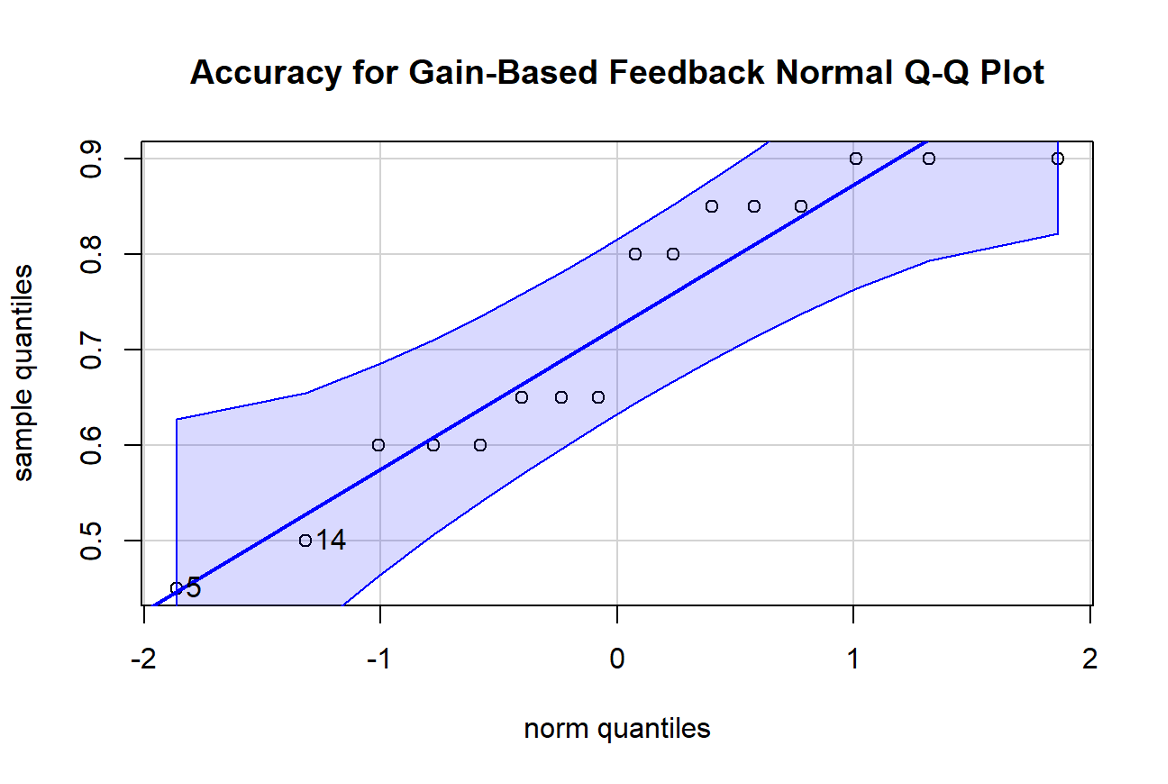
\includegraphics[width=0.8\linewidth]{images/accuracy for gain-based feedback normal Q-Q plot.png}
    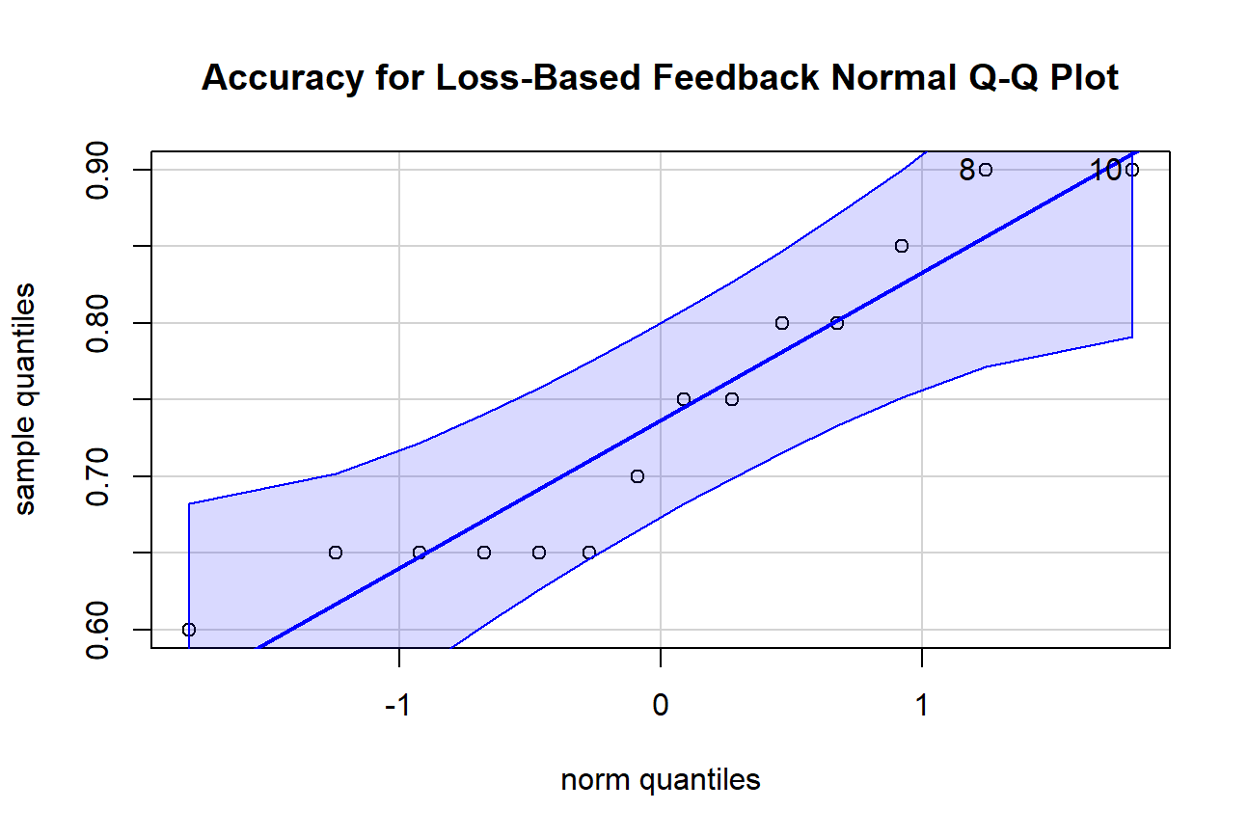
\includegraphics[width=0.8\linewidth]{images/accuracy for loss-based feedback q-q plot.png}
\end{figure}
\begin{figure}[H]
    \centering
    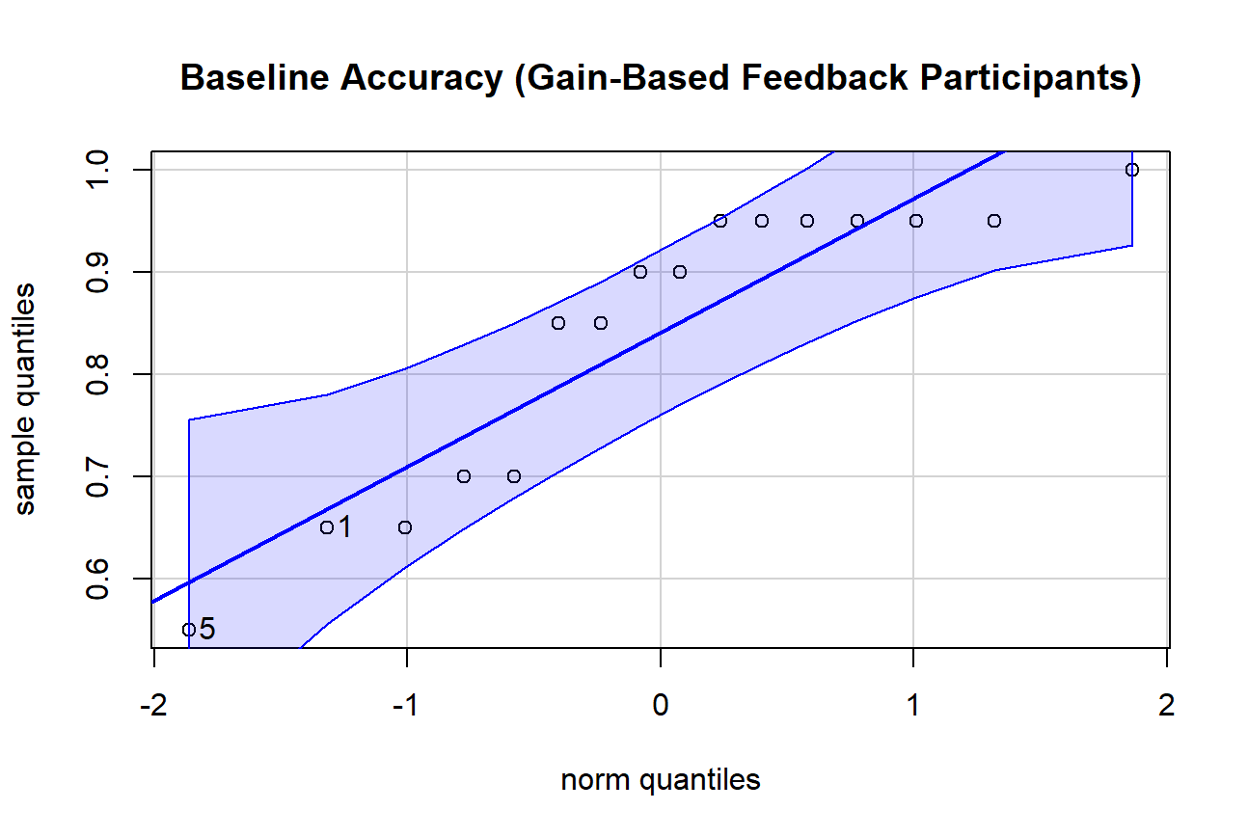
\includegraphics[width=0.8\linewidth]{images/baseline accuracy (gain based participants).png}
    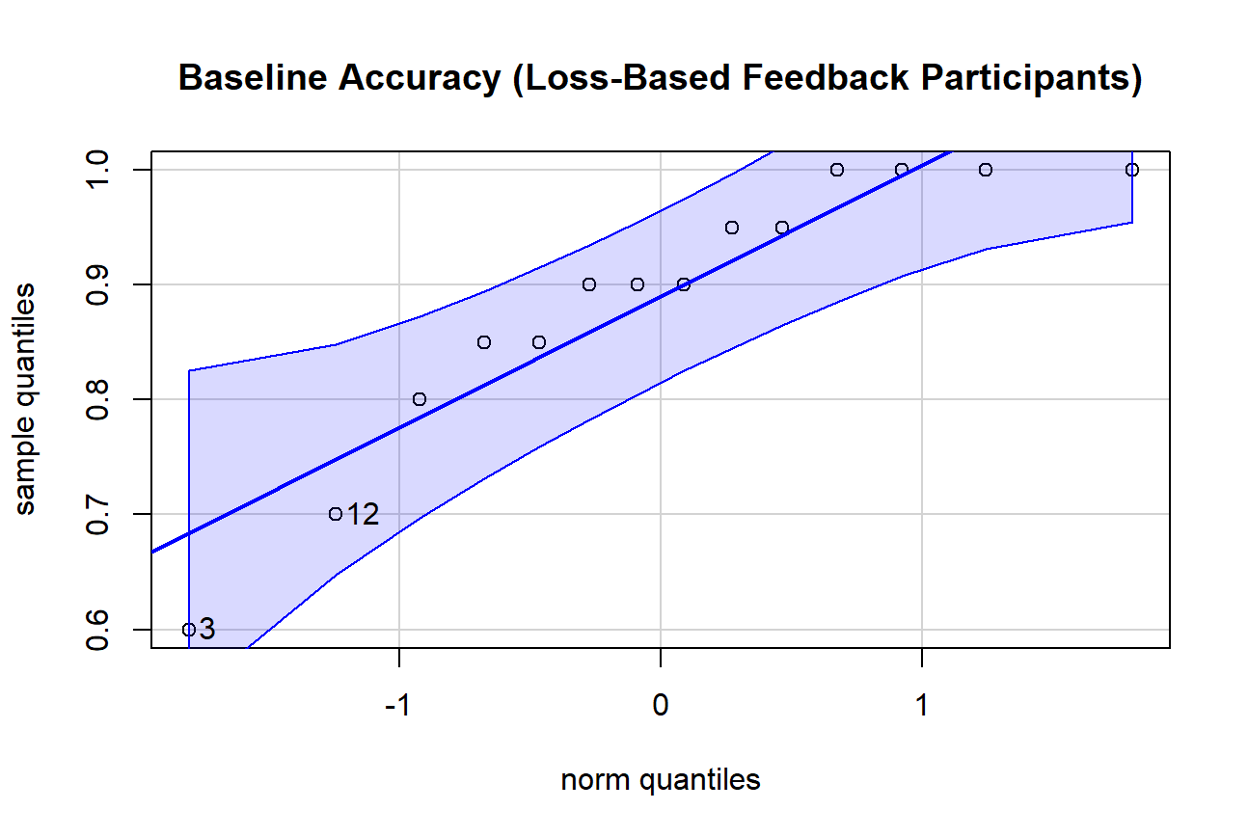
\includegraphics[width=0.8\linewidth]{images/baseline accuracy (loss-based participants).png}
\end{figure}
\begin{figure}[H]
    \centering
    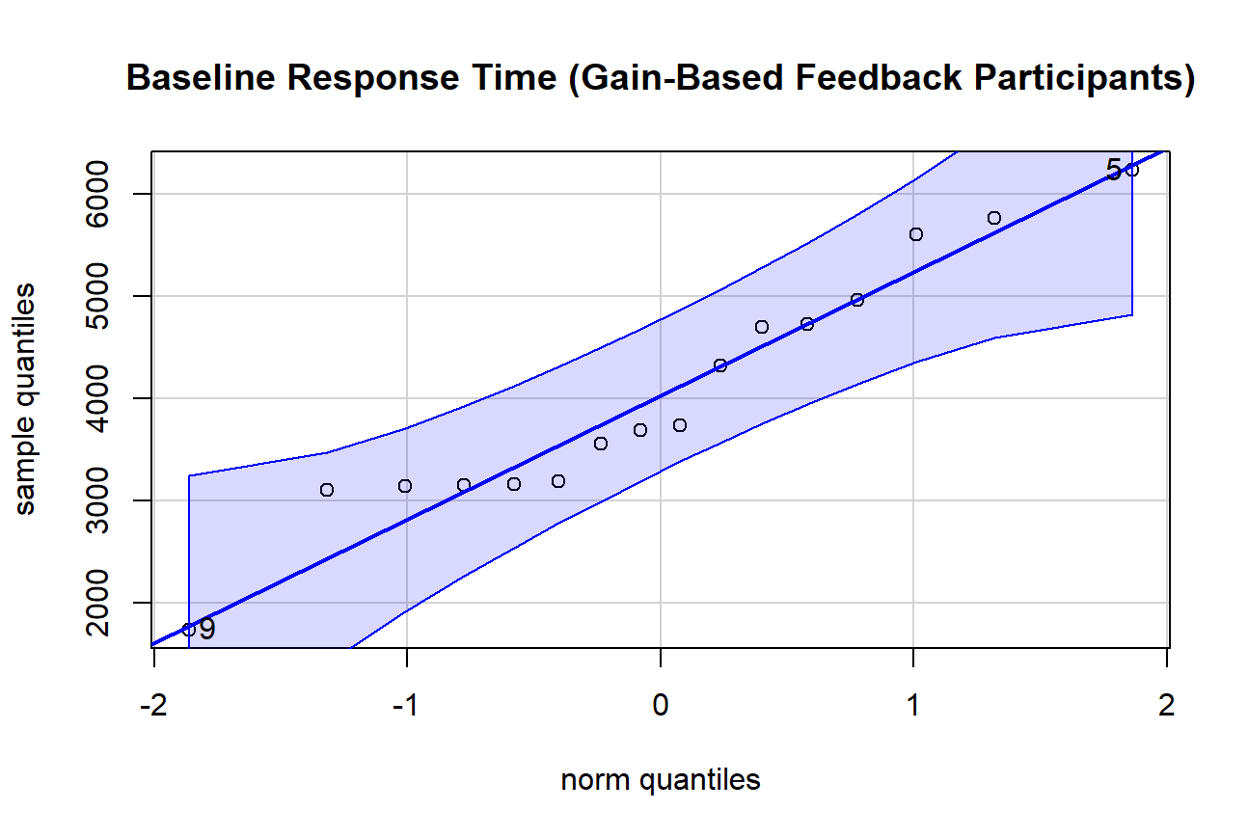
\includegraphics[width=0.8\linewidth]{images/baseline response time (gain-based participants).png}
    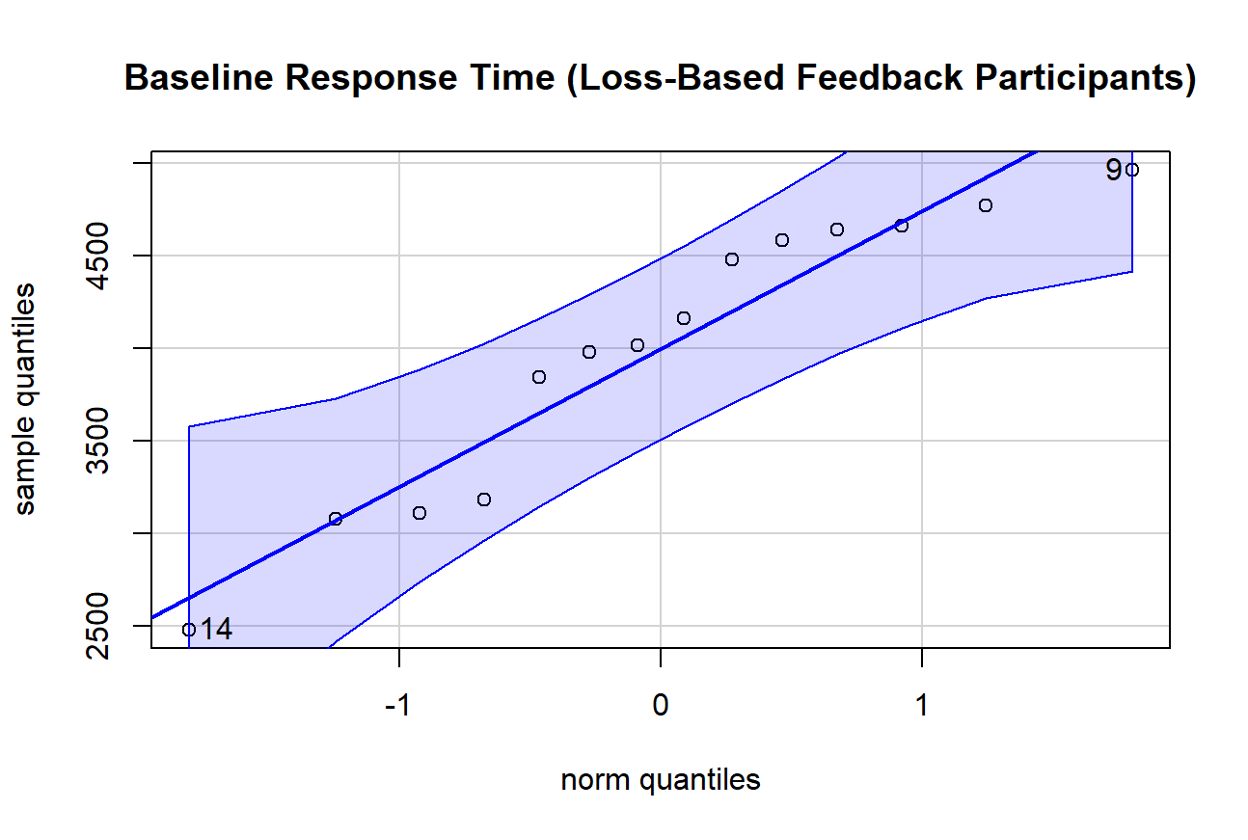
\includegraphics[width=0.8\linewidth]{images/baseline response time (loss-based participants).png}
\end{figure}
\begin{figure}[H]
    \centering
    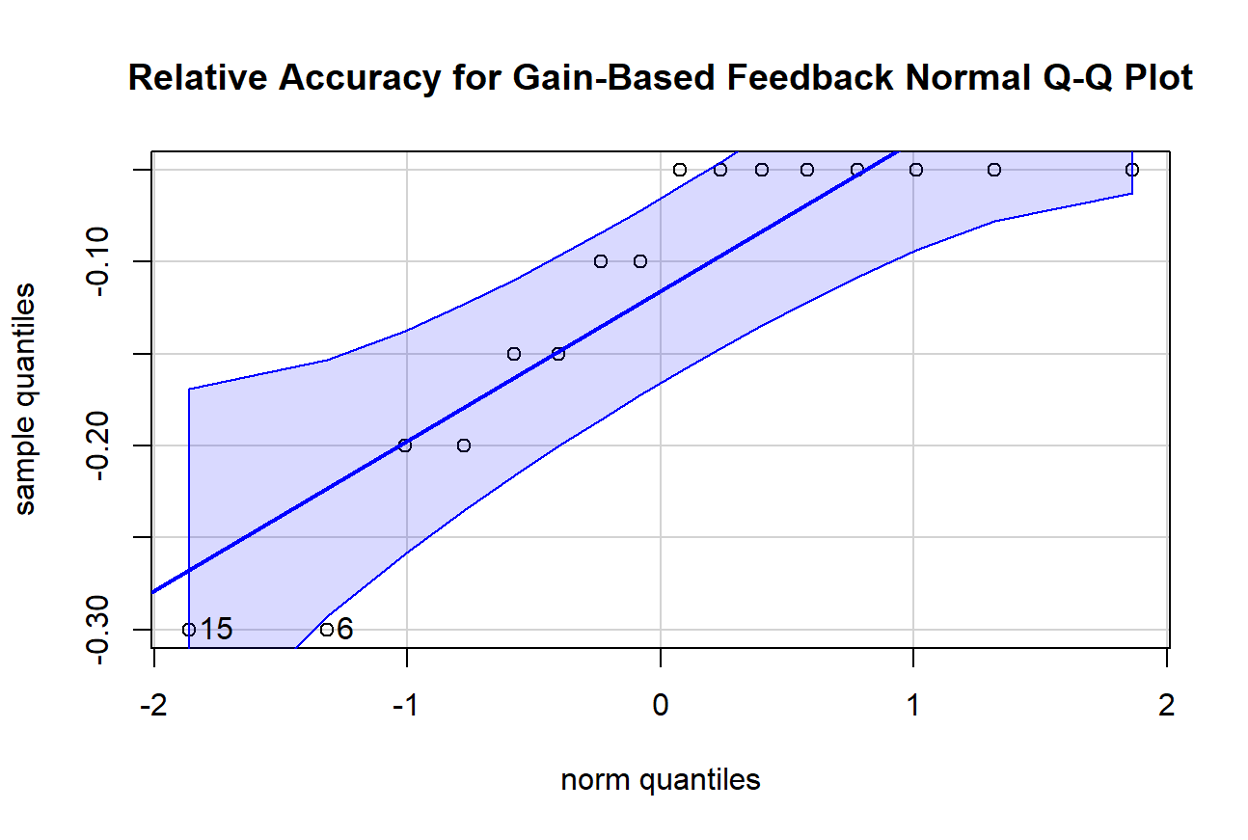
\includegraphics[width=0.8\linewidth]{images/relative accuracy gain-based feedback normal q-q.png}
    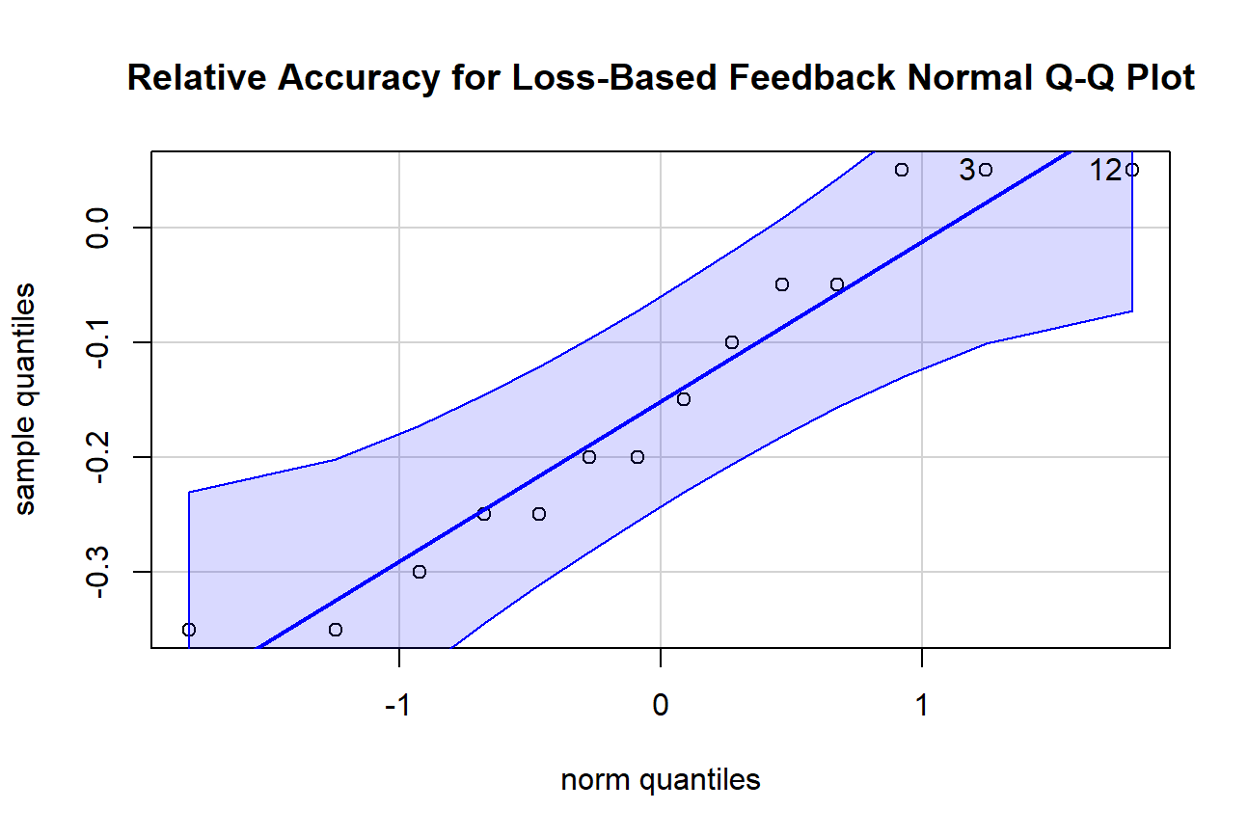
\includegraphics[width=0.8\linewidth]{images/relative accuracy loss-based feedback q-q.png}
\end{figure}
\begin{figure}[H]
    \centering
    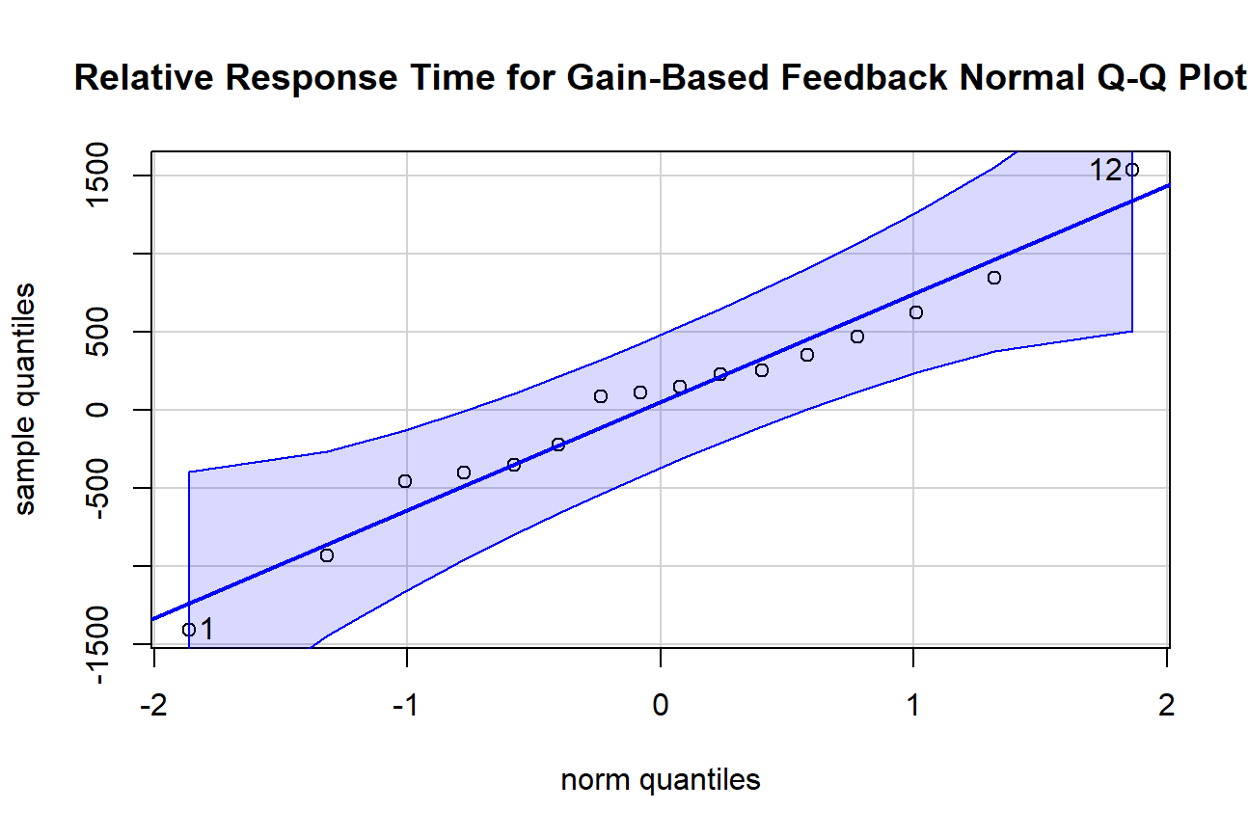
\includegraphics[width=0.8\linewidth]{images/relative response time (gain based).png}
    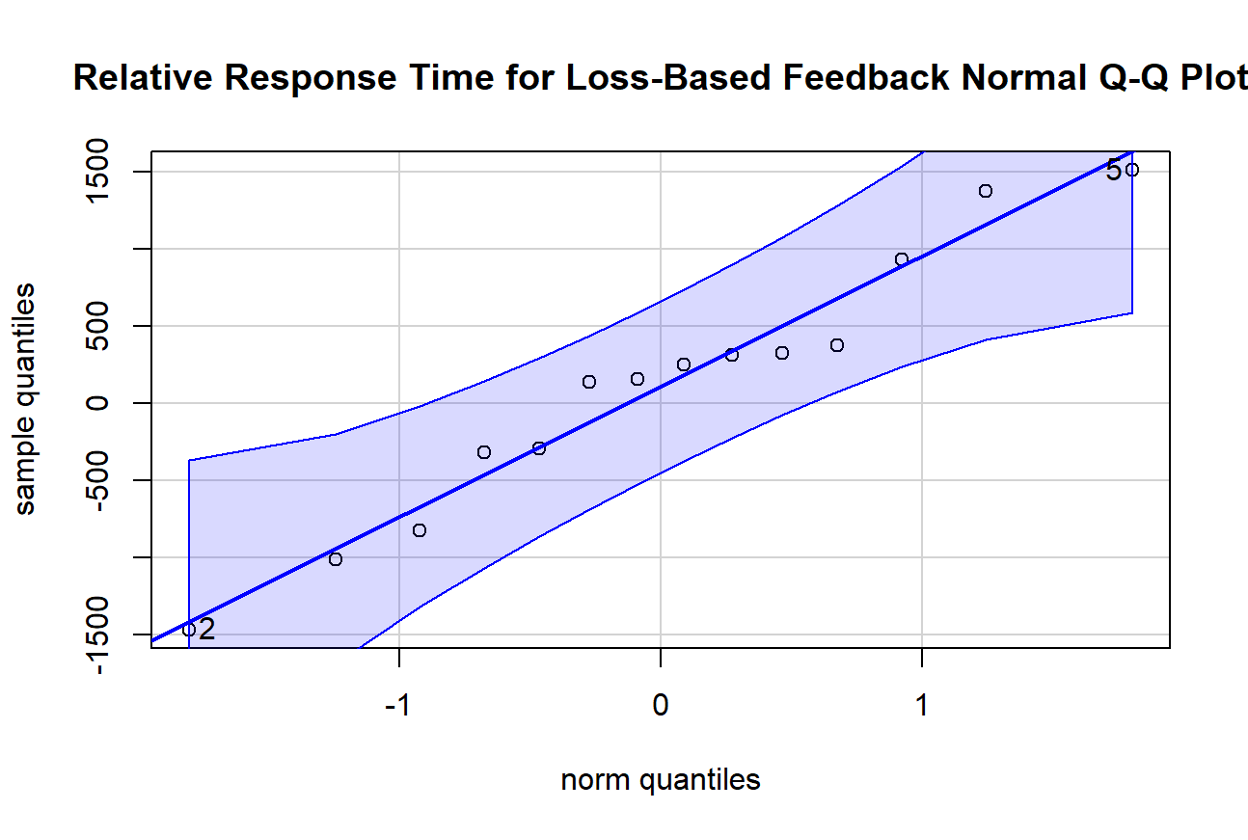
\includegraphics[width=0.8\linewidth]{images/relative response time (loss-based).png}
\end{figure}
\begin{figure}[H]
    \centering
    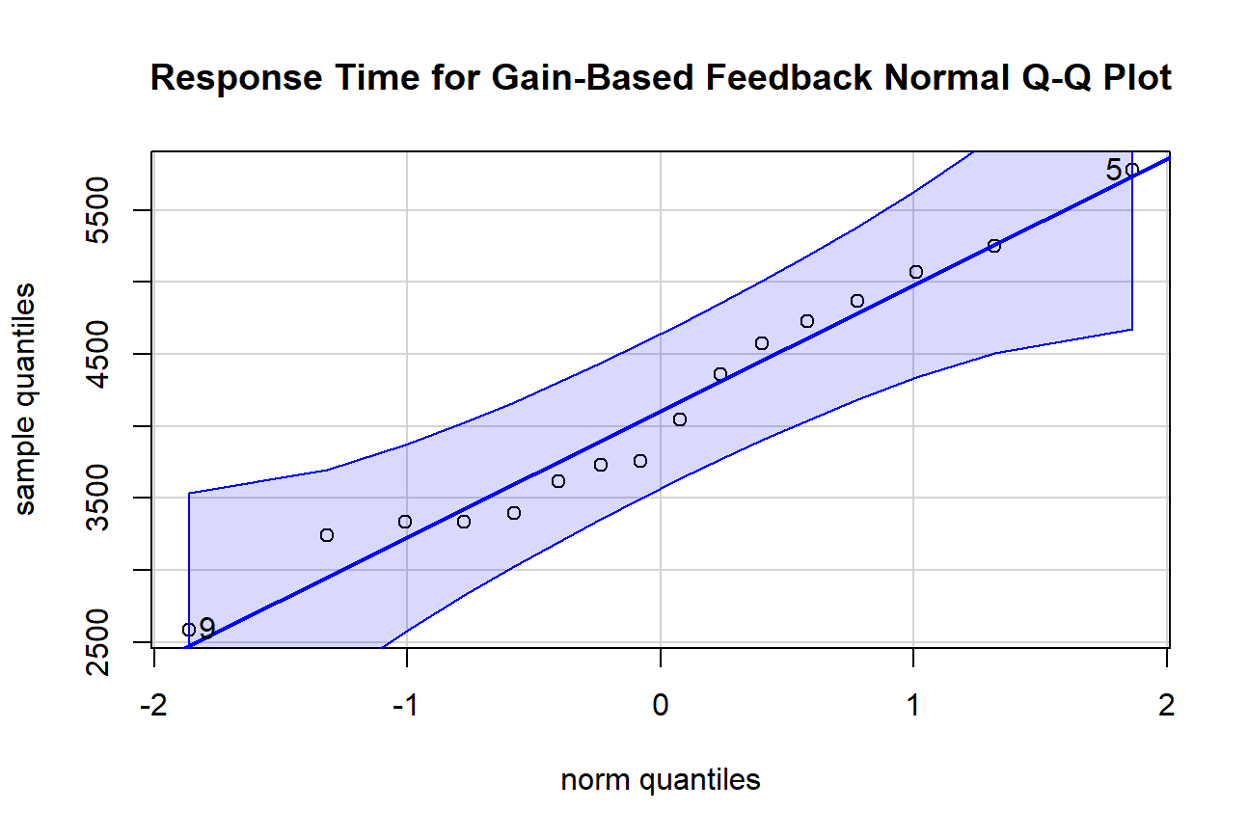
\includegraphics[width=0.8\linewidth]{images/response time (gain based).png}
    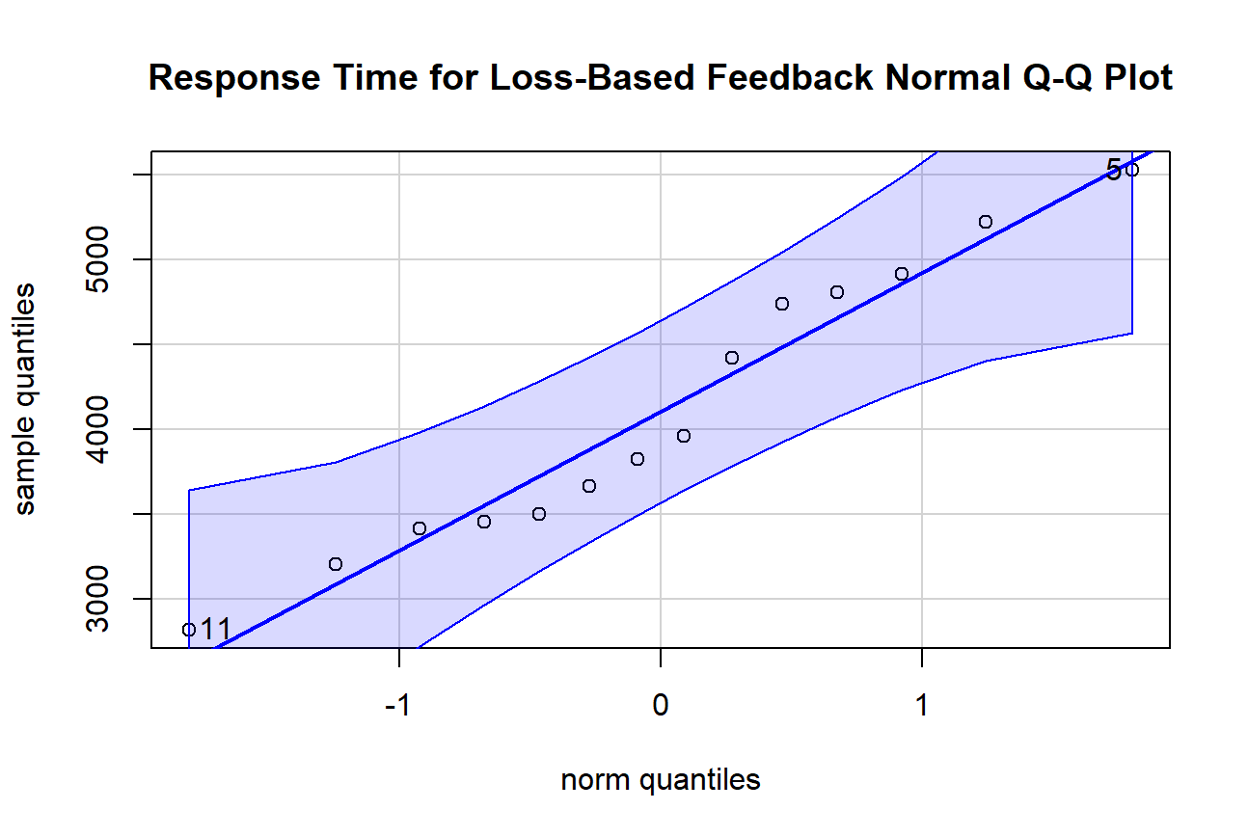
\includegraphics[width=0.8\linewidth]{images/response time (loss based).png}
\end{figure}

\section{Script for Participants}
\definecolor{readablegreen}{HTML}{006400}
\label{appdx:script}
\textit{Lines beginning with a ‘*’ are instructions to the experimenter, not instructions for participants.}

\textbf{1. BASELINE TEST:}

“To begin, you are going to be given a series of mental math questions. The questions are multiple choice and will be displayed on the screen one at a time. When shown a question, you should click the correct answer on the screen. The options will be on the screen and time remaining for the question will be in the corner. We won’t tell you how many questions you will be asked, but you should try to answer them as fast as possible. Would you like me to repeat the instructions?” 

*If they ask for a repetition, repeat the instructions verbatim

*DO NOT provide any further information to the participant than the instructions above

*Once the participant is ready, make sure the interface is switched to the BASELINE test and administer the test

\textbf{2. AFTER THE BASELINE TEST:}

\textbf{If they are doing the \textcolor{readablegreen}{GAIN BASED} test:}

“We are now going to give you another series of mental math questions. The format will be the same as before, except now you will score a point for each question you answer correctly. Again, we will not tell you how many questions you will be asked, but you should try to answer them as fast as possible and try to score as many points as possible. Would you like me to repeat the instructions?”

*If they ask for a repetition, repeat the instructions verbatim

*Once the participant is ready, switch the interface to the GAIN BASED test and administer the test

\textbf{If they are doing the \textcolor{red}{LOSS BASED} test:}

“We are now going to give you another series of mental math questions. The format will be the same as before, except now you will start with 20 points and will lose a point for each question you answer incorrectly. Again, we will not tell you how many questions you will be asked, but you should try to answer them as fast as possible while losing as few points as possible. Would you like me to repeat the instructions?”

*If they ask for a repetition, repeat the instructions verbatim

*Once the participant is ready, switch the interface to the LOSS BASED test and administer the test

\section{R code for preprocessing the raw data}
\label{appdx:r-preprocessing}
Since each participant completed 20 baseline questions and 20 feedback questions (either gain-based or loss based), we first computed the mean accuracy and response time for each participant. This reduces by-trial variability (such as random guessing or lapses in attention). This is particularly important given the relatively small number of trials per condition, where single responses could otherwise disproportionately affect the results.

\definecolor{backcolour}{rgb}{0.95,0.95,0.92}

\begin{minted}[bgcolor=backcolour, fontsize=\footnotesize, style = tango, linenos]{r}
library(jsonlite)

# all data was stored in the data/ subdirectory
DATA_PATH <- "data"

# For a given feedback type, we want to extract all the baseline results (with no feedback)
# and the actual results (with feedback)
# splitting by feedback type makes it easier to place things in an array
get_data <- function(feedback_type) {
  # data was split in to gain_data and loss_data, so load from the appropriate one
  path <- file.path(DATA_PATH, paste0(feedback_type, "_data"))
  # get all files in the directory
  files <- list.files(path)
  # for debugging to ensure we got all of them
  print(files)
  
  # to store the processed output
  results <- list()
  
  for (file in files) {
    # if for some reason a file is incorrectly named, skip it (e.g., old testing files)
    if (!grepl(feedback_type, file)) {
      next
    }
    
    # get the name of the participant
    name <- strsplit(file, "_")[[1]][1]
    # get their baseline file
    baseline_file <- paste0(name, "_baseline.json")
    
    # load data as a dataframe from the json files
    feedback_data <- fromJSON(file.path(path, file))
    baseline_data <- fromJSON(file.path(path, baseline_file))
    
    # append it to the array (by inserting at the current length + 1)
    results[[length(results) + 1]] <- list(
      baseline = baseline_data,
      feedback = feedback_data
    )
  }
  
  # output the array, where each entry is
  # the baseline + feedback data for a given participant
  return(results)
}

process <- function(feedback_type) {
  # get the data
  data <- get_data(feedback_type)
  
  # arrays to store the scores
  baseline_scores <- c()
  baseline_times <- c()
  feedback_scores <- c()
  feedback_times <- c()
  
  for (participant in data) {
    # load the individual data from the dataframes
    baseline <- participant$baseline
    feedback <- participant$feedback
    
    # compute the mean score and time taken in the baseline case
    baseline_score <- mean((baseline$correct))
    baseline_time <- mean((baseline$time_taken))
    
    # repeat for the feedback case
    feedback_score <- mean((feedback$correct))
    feedback_time <- mean((feedback$time_taken))
    
    # add these to the array
    baseline_scores <- c(baseline_scores, baseline_score)
    baseline_times <- c(baseline_times, baseline_time)
    feedback_scores <- c(feedback_scores, feedback_score)
    feedback_times <- c(feedback_times, feedback_time)
  }
  
  # output the data
  return(list(
    baseline_scores = baseline_scores,
    baseline_times = baseline_times,
    feedback_scores = feedback_scores,
    feedback_times = feedback_times
  ))
}

write_file <- function(filename) {
  # the main file that processes our raw data into a new JSON file
  # (which can then be read by the analysis R code)
  gain <- process("gain")  # get gain data
  loss <- process("loss")  # get loss data
  
  # now we're just rearranging the arrays and mapping them to useful keys
  # this way in the analysis R code, we can import this as a dataframe
  # and have access to arrays of relevant data
  # for example, doing data$gain_baseline_accuracy will
  # give us a list of all baseline accuracies
  # (on a scale from 0 to 1)
  # which we could then, say, plot on a QQ-norm plot
  result <- list(
    gain_baseline_accuracy = gain$baseline_scores,
    gain_baseline_response_time = gain$baseline_times,
    gain_feedback_accuracy = gain$feedback_scores,
    gain_feedback_response_time = gain$feedback_times,
    
    loss_baseline_accuracy = loss$baseline_scores,
    loss_baseline_response_time = loss$baseline_times,
    loss_feedback_accuracy = loss$feedback_scores,
    loss_feedback_response_time = loss$feedback_times
  )
  
  # write the data to a file
  # pretty = TRUE makes it more human readable
  # (adding line breaks, etc. instead of one long string)
  # this doesn't affect the data in any way
  # but it makes it easier for us to check
  write_json(result, filename, pretty = TRUE, auto_unbox = TRUE)
}

# call the function to actually do the analysis
write_file("averaged_data.json")
\end{minted}

\section{R code for analysis}
\begin{minted}[bgcolor=backcolour, fontsize=\footnotesize, style = tango, linenos]{r}
install.packages("rjson")
library("rjson")
install.packages("car")
library(car)

# Loading data from the JSON file
averaged_data <- fromJSON(file = "averaged_data.json")

attach(averaged_data)

# Defining relative scores
relative_gain_feedback_accuracy = gain_feedback_accuracy - gain_baseline_accuracy
relative_gain_feedback_response_time = gain_feedback_response_time - gain_baseline_response_time
relative_loss_feedback_accuracy = loss_feedback_accuracy - loss_baseline_accuracy
relative_loss_feedback_response_time = loss_feedback_response_time - loss_baseline_response_time

# Q-Q plots

## Baselines
qqPlot(gain_baseline_accuracy, distribution = "norm", 
       main = "Baseline Accuracy (Gain-Based Feedback Participants)",
       ylab = "sample quantiles",
       envelope=0.95,
       line = c("robust"))
qqPlot(gain_baseline_response_time, distribution = "norm", 
       main = "Baseline Response Time (Gain-Based Feedback Participants)",
       ylab = "sample quantiles",
       envelope=0.95,
       line = c("robust"))
qqPlot(loss_baseline_accuracy, distribution = "norm", 
       main = "Baseline Accuracy (Loss-Based Feedback Participants)",
       ylab = "sample quantiles",
       envelope=0.95,
       line = c("robust"))
qqPlot(loss_baseline_response_time, distribution = "norm", 
       main = "Baseline Response Time (Loss-Based Feedback Participants)",
       ylab = "sample quantiles",
       envelope=0.95,
       line = c("robust"))

## GAIN
qqPlot(gain_feedback_accuracy, distribution = "norm", 
       main = "Accuracy for Gain-Based Feedback Normal Q-Q Plot",
       ylab = "sample quantiles",
       envelope=0.95,
       line = c("robust"))
qqPlot(gain_feedback_response_time, distribution = "norm", 
       main = "Response Time for Gain-Based Feedback Normal Q-Q Plot",
       ylab = "sample quantiles",
       envelope=0.95,
       line = c("robust"))

qqPlot(relative_gain_feedback_accuracy, distribution = "norm", 
       main = "Relative Accuracy for Gain-Based Feedback Normal Q-Q Plot",
       ylab = "sample quantiles",
       envelope=0.95,
       line = c("robust"))
qqPlot(relative_gain_feedback_response_time, distribution = "norm", 
       main = "Relative Response Time for Gain-Based Feedback Normal Q-Q Plot",
       ylab = "sample quantiles",
       envelope=0.95,
       line = c("robust"))

## LOSS
qqPlot(loss_feedback_accuracy, distribution = "norm", 
       main = "Accuracy for Loss-Based Feedback Normal Q-Q Plot",
       ylab = "sample quantiles",
       envelope=0.95,
       line = c("robust"))
qqPlot(loss_feedback_response_time, distribution = "norm", 
       main = "Response Time for Loss-Based Feedback Normal Q-Q Plot",
       ylab = "sample quantiles",
       envelope=0.95,
       line = c("robust"))
qqPlot(relative_loss_feedback_accuracy, distribution = "norm", 
       main = "Relative Accuracy for Loss-Based Feedback Normal Q-Q Plot",
       ylab = "sample quantiles",
       envelope=0.95,
       line = c("robust"))
qqPlot(relative_loss_feedback_response_time, distribution = "norm", 
       main = "Relative Response Time for Loss-Based Feedback Normal Q-Q Plot",
       ylab = "sample quantiles",
       envelope=0.95,
       line = c("robust"))

# One-sided t-tests

## Loss vs. baseline
t.test(loss_feedback_accuracy, loss_baseline_accuracy,
       alternative = c("greater"), paired=TRUE)
t.test(loss_feedback_response_time, loss_baseline_response_time,
       alternative = c("greater"), paired=TRUE)

## Gain vs. baseline
t.test(gain_feedback_accuracy, gain_baseline_accuracy,
       alternative = c("greater"), paired=TRUE)
t.test(gain_feedback_response_time, gain_baseline_response_time,
       alternative = c("greater"), paired=TRUE)

## Loss vs. Gain
t.test(loss_feedback_accuracy, gain_feedback_accuracy[1:14], 
       alternative = c("greater"), paired=FALSE)
t.test(relative_loss_feedback_accuracy, relative_gain_feedback_accuracy[1:14], 
       alternative = c("greater"), paired=FALSE)
t.test(loss_feedback_response_time, gain_feedback_response_time[1:14], 
       alternative = c("greater"), paired=FALSE)
t.test(relative_loss_feedback_response_time, relative_gain_feedback_response_time[1:14], 
       alternative = c("greater"), paired=FALSE)

# Two-sided t-tests

## Loss vs. baseline
t.test(loss_feedback_accuracy, loss_baseline_accuracy,
       alternative = c("two.sided"), paired=TRUE)
t.test(loss_feedback_response_time, loss_baseline_response_time,
       alternative = c("two.sided"), paired=TRUE)

## Gain vs. baseline
t.test(gain_feedback_accuracy, gain_baseline_accuracy,
       alternative = c("two.sided"), paired=TRUE)
t.test(gain_feedback_response_time, gain_baseline_response_time,
       alternative = c("two.sided"), paired=TRUE)

## Loss vs. Gain
t.test(loss_feedback_accuracy, gain_feedback_accuracy[1:14], 
       alternative = c("two.sided"), paired=FALSE)
t.test(relative_loss_feedback_accuracy, relative_gain_feedback_accuracy[1:14], 
       alternative = c("two.sided"), paired=FALSE)
t.test(loss_feedback_response_time, gain_feedback_response_time[1:14], 
       alternative = c("two.sided"), paired=FALSE)
t.test(relative_loss_feedback_response_time, relative_gain_feedback_response_time[1:14], 
       alternative = c("two.sided"), paired=FALSE)

# Histograms

## GAIN
hist(gain_baseline_accuracy, 
     main = paste("Accuracy for Baseline Trials (Gain-Based Feedback Participants)"),
     xlab =  "Accuracy", axes = TRUE, plot = TRUE)
hist(gain_feedback_accuracy, 
     main = paste("Accuracy for Gain-Based Feedback Trials"),
     xlab =  "Accuracy", axes = TRUE, plot = TRUE)
hist(gain_baseline_response_time, 
     main = paste("Response Time for Baseline Trials (Gain-Based Feedback Participants)"),
     xlab =  "Accuracy", axes = TRUE, plot = TRUE)
hist(gain_feedback_response_time, 
     main = paste("Response Time for Gain-Based Feedback Trials"),
     xlab =  "Accuracy", axes = TRUE, plot = TRUE)

hist(relative_gain_feedback_accuracy, 
     main = paste("Relative Accuracy for Gain-Based Feedback Trials"),
     xlab =  "Accuracy", axes = TRUE, plot = TRUE)
hist(relative_gain_feedback_response_time, 
     main = paste("Relative Response Time for Gain-Based Feedback Trials"),
     xlab =  "Accuracy", axes = TRUE, plot = TRUE)

## LOSS
hist(loss_baseline_accuracy, 
     main = paste("Accuracy for Baseline Trials (Loss-Based Feedback Participants)"),
     xlab =  "Accuracy", axes = TRUE, plot = TRUE)
hist(loss_feedback_accuracy, 
     main = paste("Accuracy for Loss-Based Feedback Trials"),
     xlab =  "Accuracy", axes = TRUE, plot = TRUE)
hist(loss_baseline_response_time, 
     main = paste("Response Time for Baseline Trials (Loss-Based Feedback Participants)"),
     xlab =  "Accuracy", axes = TRUE, plot = TRUE)
hist(loss_feedback_response_time, 
     main = paste("Response Time for Loss-Based Feedback Trials"),
     xlab =  "Accuracy", axes = TRUE, plot = TRUE)

hist(relative_loss_feedback_accuracy, 
     main = paste("Relative Accuracy for Loss-Based Feedback Trials"),
     xlab =  "Accuracy", axes = TRUE, plot = TRUE)
hist(relative_loss_feedback_response_time, 
     main = paste("Relative Response Time for Loss-Based Feedback Trials"),
     xlab =  "Accuracy", axes = TRUE, plot = TRUE)


# Box Plots 

par(mfrow = c(1, 2)) 
 
boxplot(gain_feedback_accuracy, loss_feedback_accuracy,
        names = c("Gain", "Loss"),
        main = "Accuracy by Feedback Type (Absolute)",
        ylab = "Accuracy",
        col = c("lightblue", "lightcoral"))

stripchart(list(gain_feedback_accuracy, loss_feedback_accuracy),
           method = "jitter",
           pch = 16,
           col = rgb(0, 0, 0, 0.5),
           vertical = TRUE,
           add = TRUE)

boxplot(gain_feedback_response_time, loss_feedback_response_time,
        names = c("Gain", "Loss"),
        main = "Response Time by Feedback Type (Absolute)",
        ylab = "Response Time (ms)",
        col = c("lightblue", "lightcoral"))

stripchart(list(gain_feedback_response_time, loss_feedback_response_time),
           method = "jitter",
           pch = 16,
           col = rgb(0, 0, 0, 0.5),
           vertical = TRUE,
           add = TRUE)

par(mfrow = c(1, 2)) 

boxplot(relative_gain_feedback_accuracy, relative_loss_feedback_accuracy,
        names = c("Gain", "Loss"),
        main = "Accuracy by Feedback Type (Relative to Basline)",
        ylab = "Accuracy",
        col = c("lightblue", "lightcoral"))

stripchart(list(relative_gain_feedback_accuracy, relative_loss_feedback_accuracy),
           method = "jitter",
           pch = 16,
           col = rgb(0, 0, 0, 0.5),
           vertical = TRUE,
           add = TRUE)

boxplot(relative_gain_feedback_response_time, relative_loss_feedback_response_time,
        names = c("Gain", "Loss"),
        main = "Response Time by Feedback Type (Relative to Basline)",
        ylab = "Response Time (ms)",
        col = c("lightblue", "lightcoral"))

stripchart(list(relative_gain_feedback_response_time, relative_loss_feedback_response_time),
           method = "jitter",
           pch = 16,
           col = rgb(0, 0, 0, 0.5),
           vertical = TRUE,
           add = TRUE)
\end{minted}

\section{Boxplots}
\label{appdx:boxplots}
\begin{figure}[H]
    \centering
    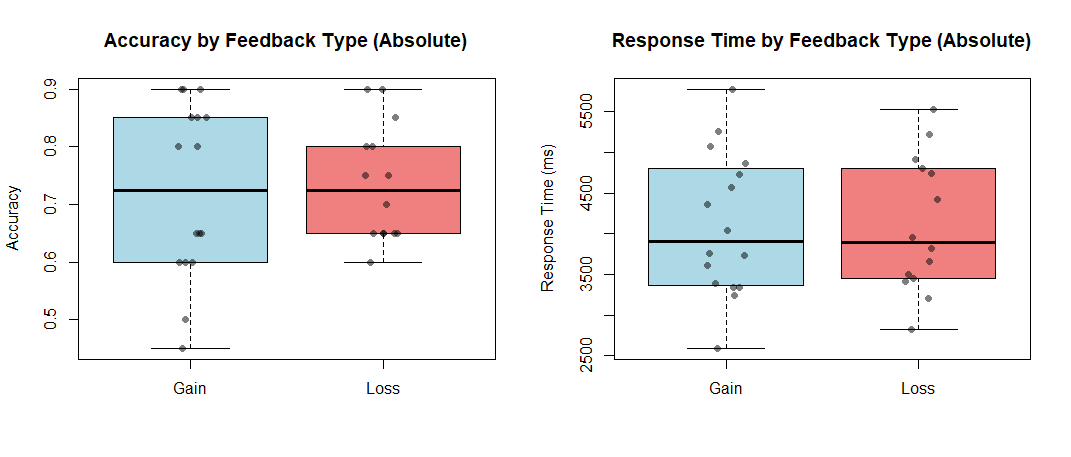
\includegraphics[width=1\linewidth]{images/boxplots of absolute accuracy and response times .png}
    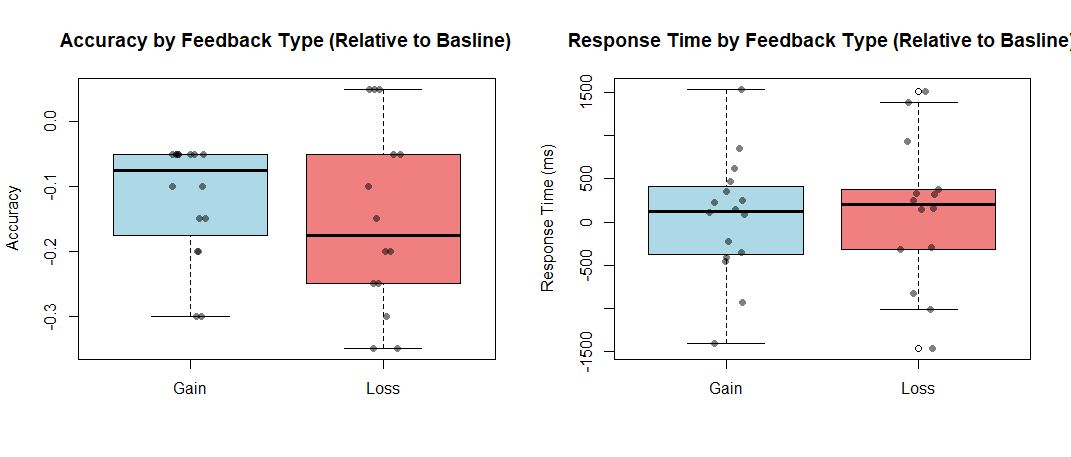
\includegraphics[width=1\linewidth]{images/boxplots of relative accuracy by feedback type.png}
\end{figure}

\section{Histograms}
\label{appdx:histograms}

\begin{figure}[H]
	\centering
	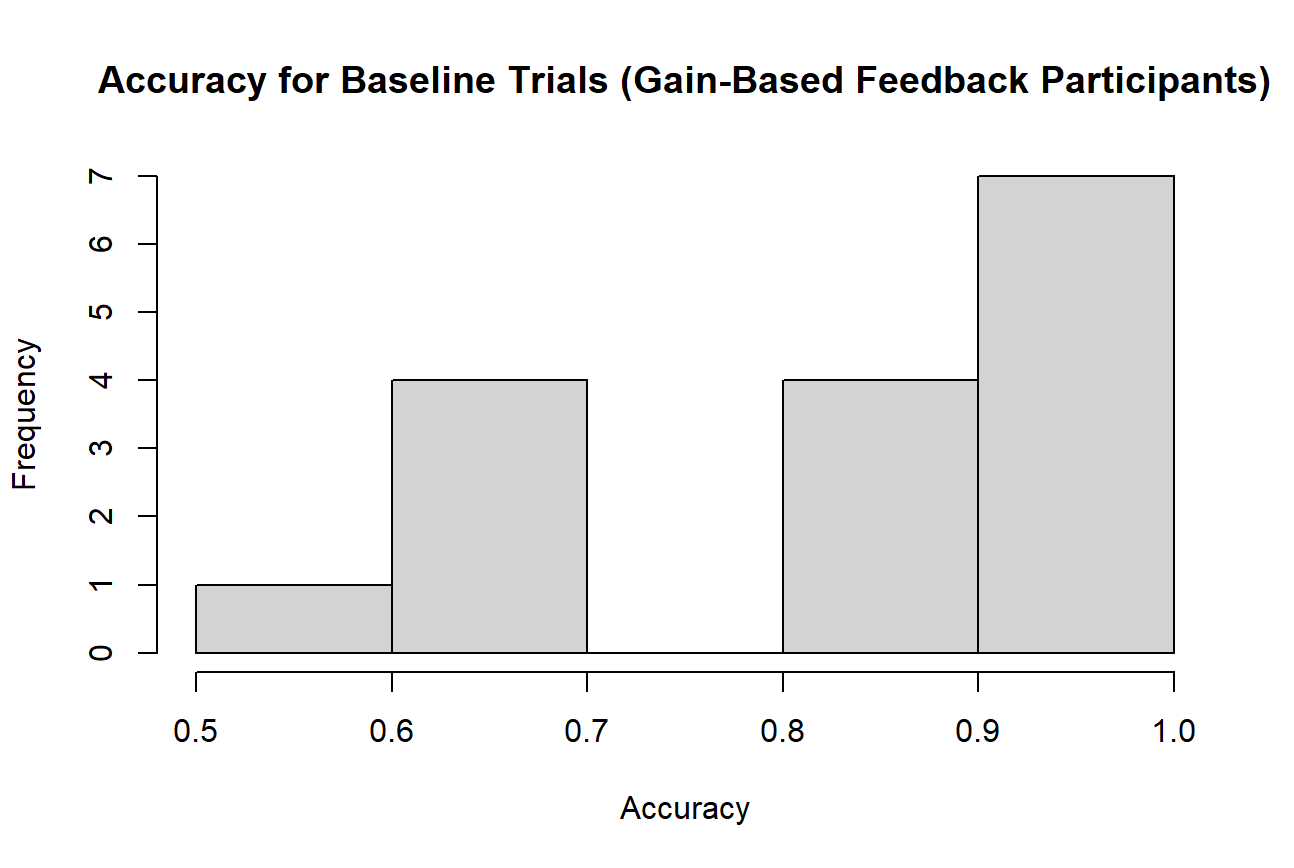
\includegraphics[width=0.8\linewidth]{images/Histograms/Accuracy for Baseline Trials (Gain-Based Feedback Participants).png}
\end{figure}
\begin{figure}[H]
	\centering
	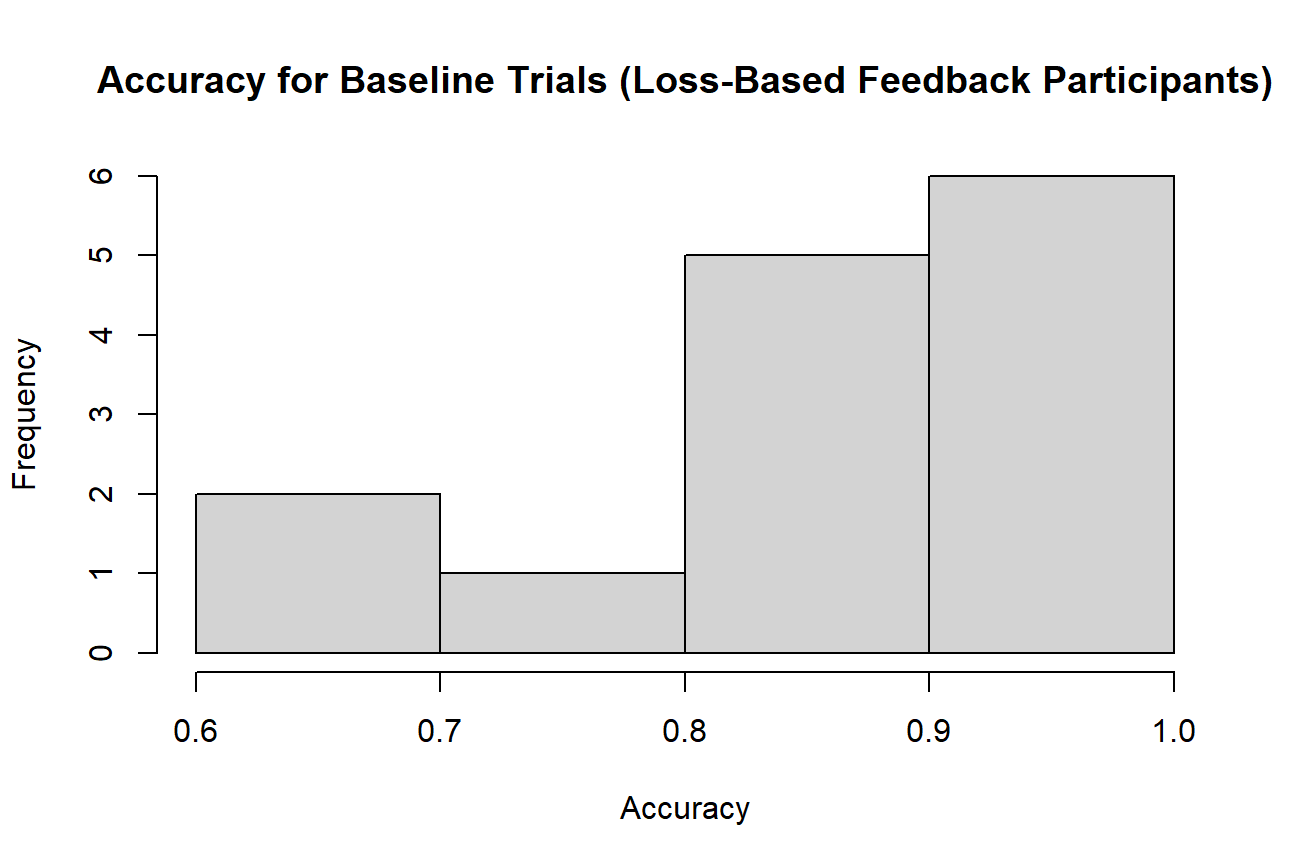
\includegraphics[width=0.8\linewidth]{images/Histograms/Accuracy for Baseline Trials (Loss-Based Feedback Participants).png}
\end{figure}
\begin{figure}[H]
	\centering
	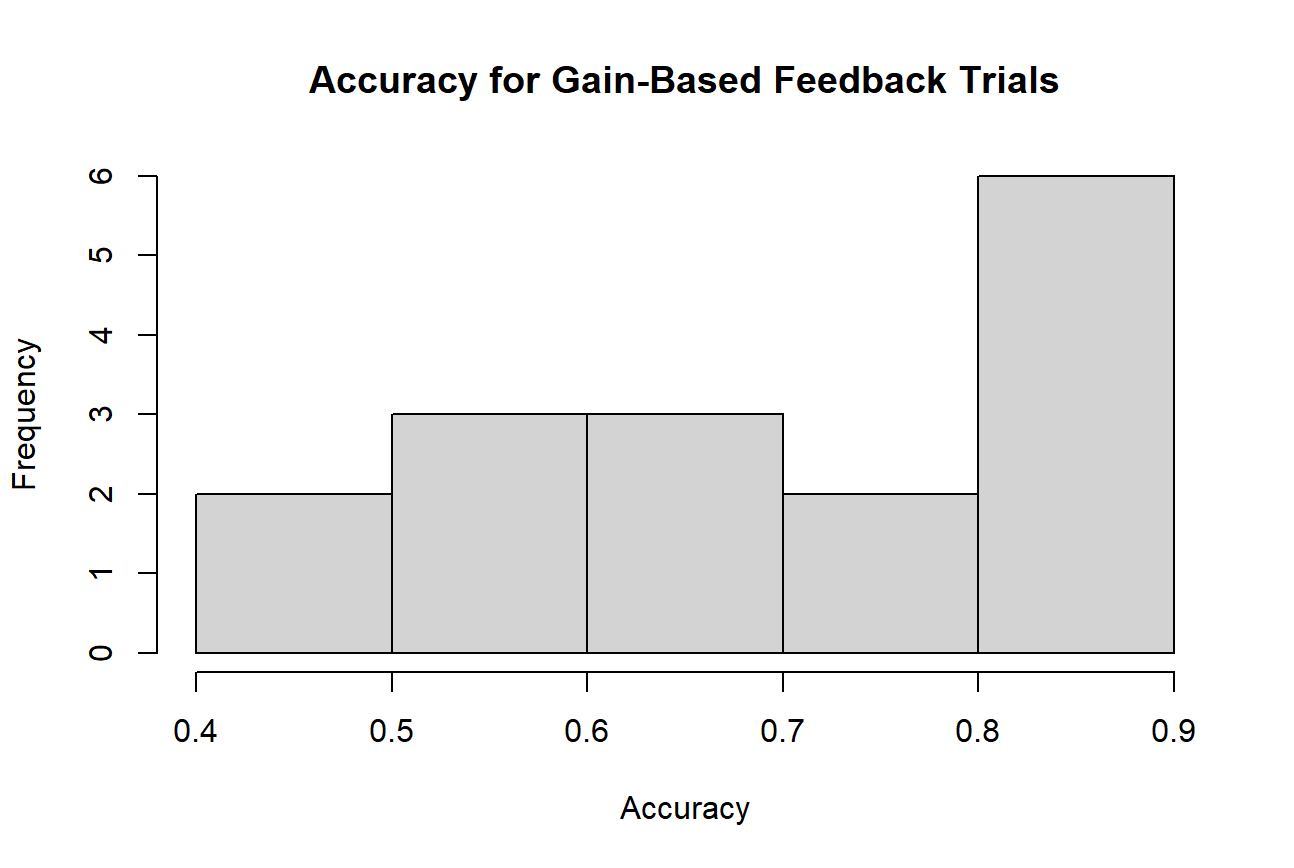
\includegraphics[width=0.8\linewidth]{images/Histograms/Accuracy for Gain-Based Feedback Trials.png}
\end{figure}
\begin{figure}[H]
	\centering
	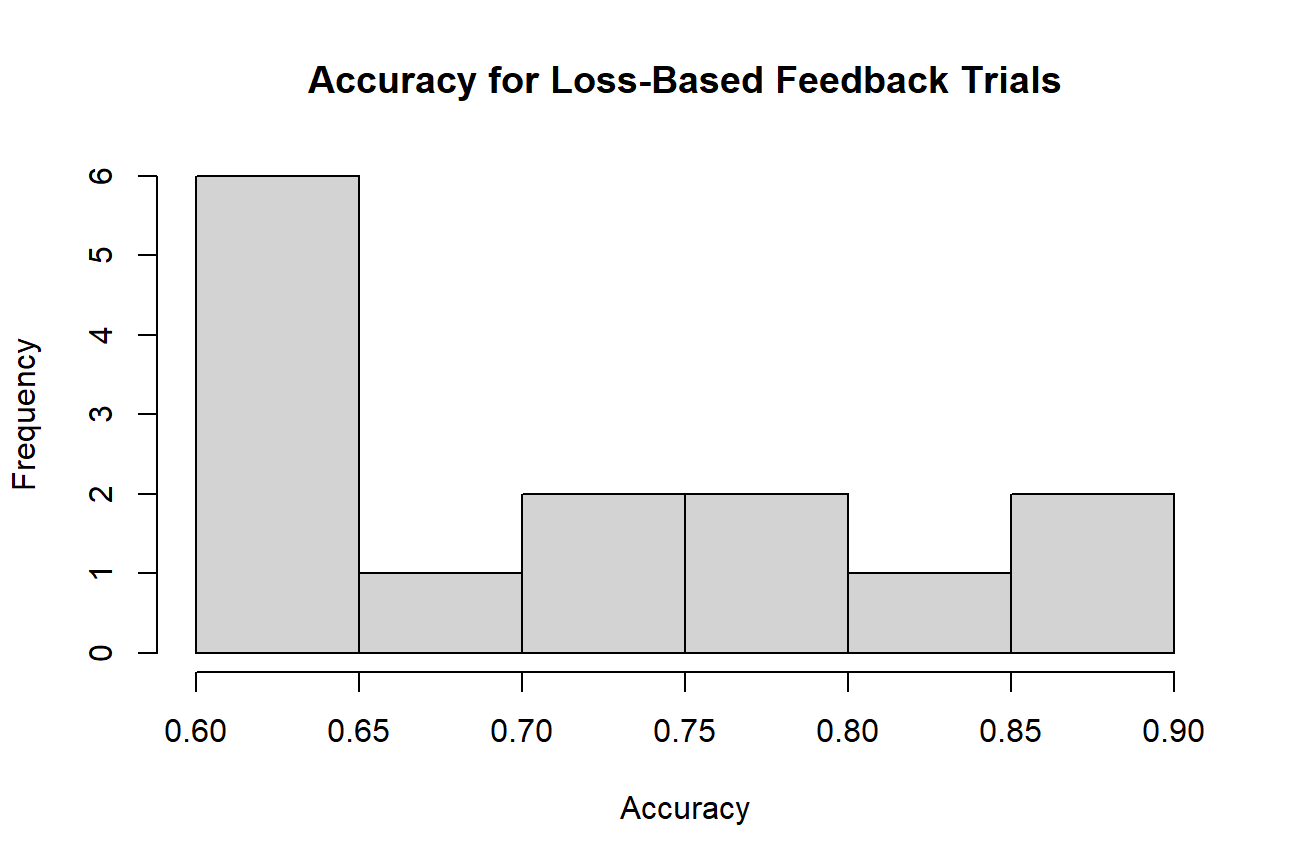
\includegraphics[width=0.8\linewidth]{images/Histograms/Accuracy for Loss-Based Feedback Trials.png}
\end{figure}
\begin{figure}[H]
	\centering
	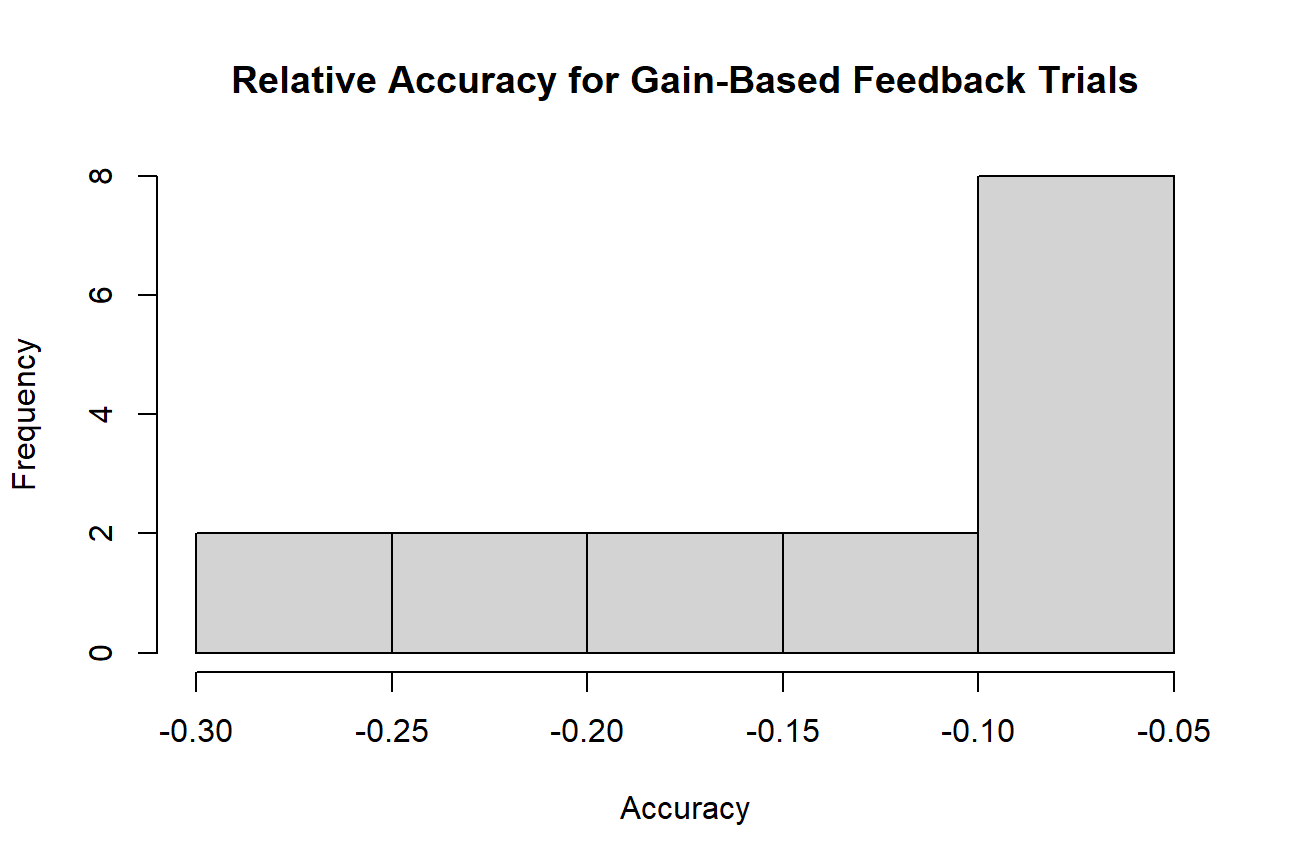
\includegraphics[width=0.8\linewidth]{images/Histograms/Relative Accuracy for Gain-Based Feedback Trials.png}
\end{figure}
\begin{figure}[H]
	\centering
	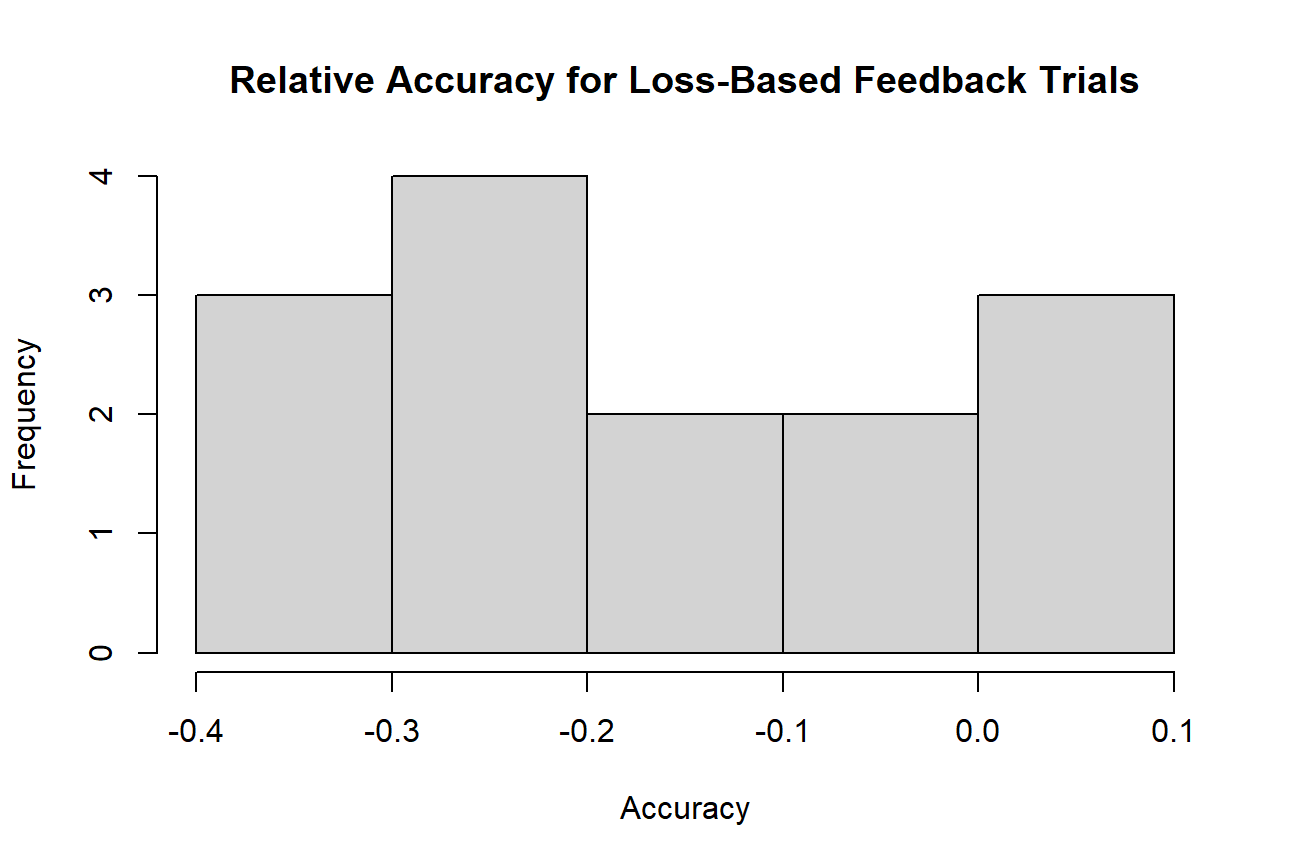
\includegraphics[width=0.8\linewidth]{images/Histograms/Relative Accuracy for Loss-Based Feedback Trials.png}
\end{figure}
\begin{figure}[H]
	\centering
	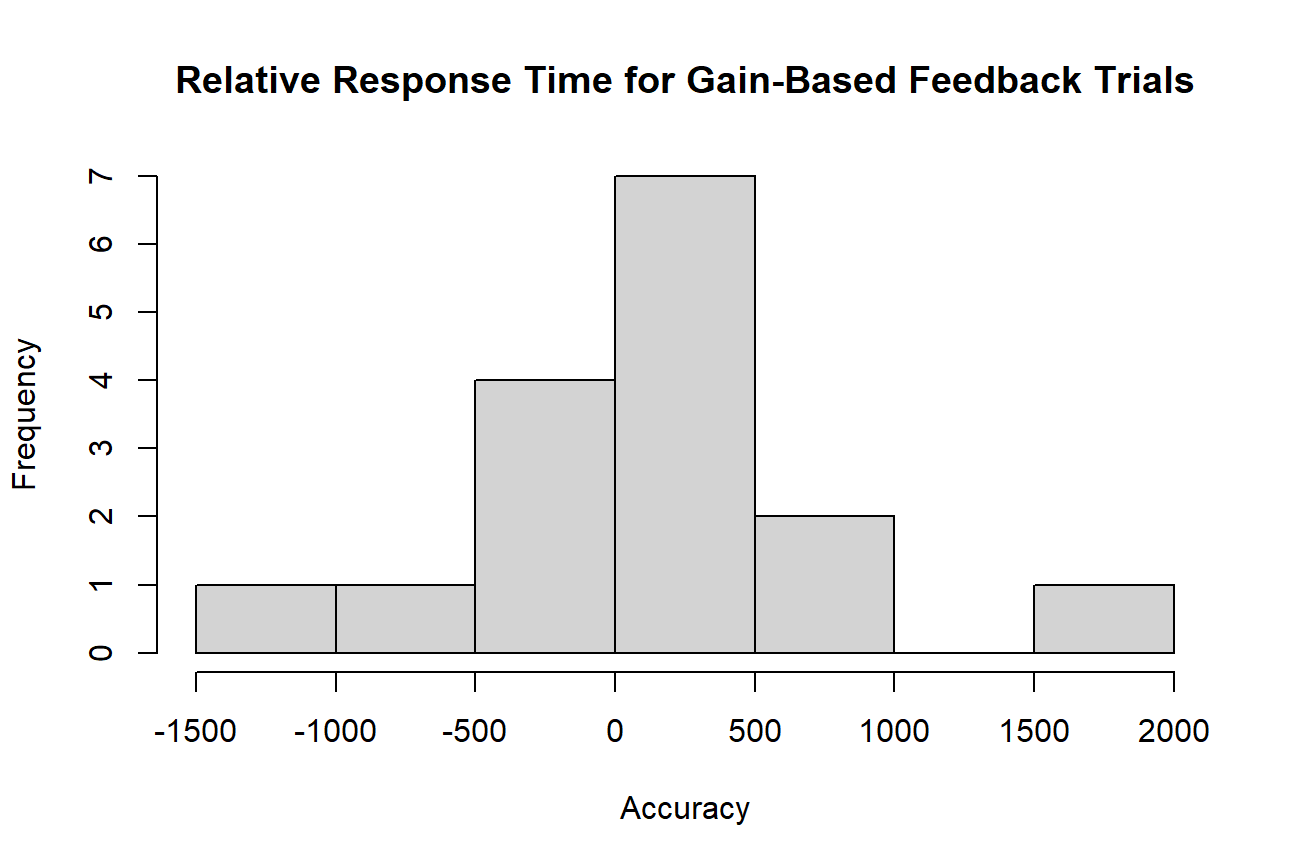
\includegraphics[width=0.8\linewidth]{images/Histograms/Relative Response Time for Gain-Based Feedback Trials.png}
\end{figure}
\begin{figure}[H]
	\centering
	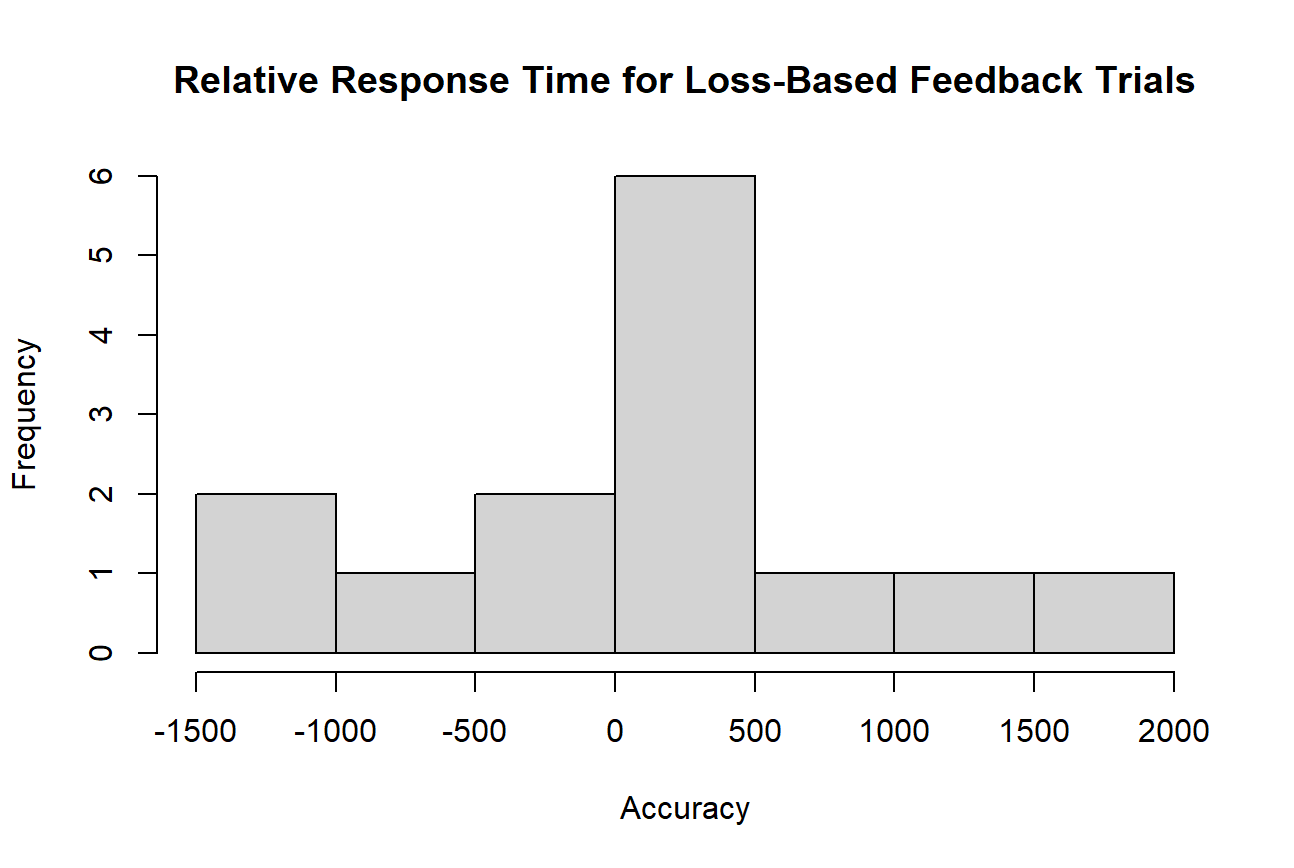
\includegraphics[width=0.8\linewidth]{images/Histograms/Relative Response Time for Loss-Based Feedback Trials.png}
\end{figure}
\begin{figure}[H]
	\centering
	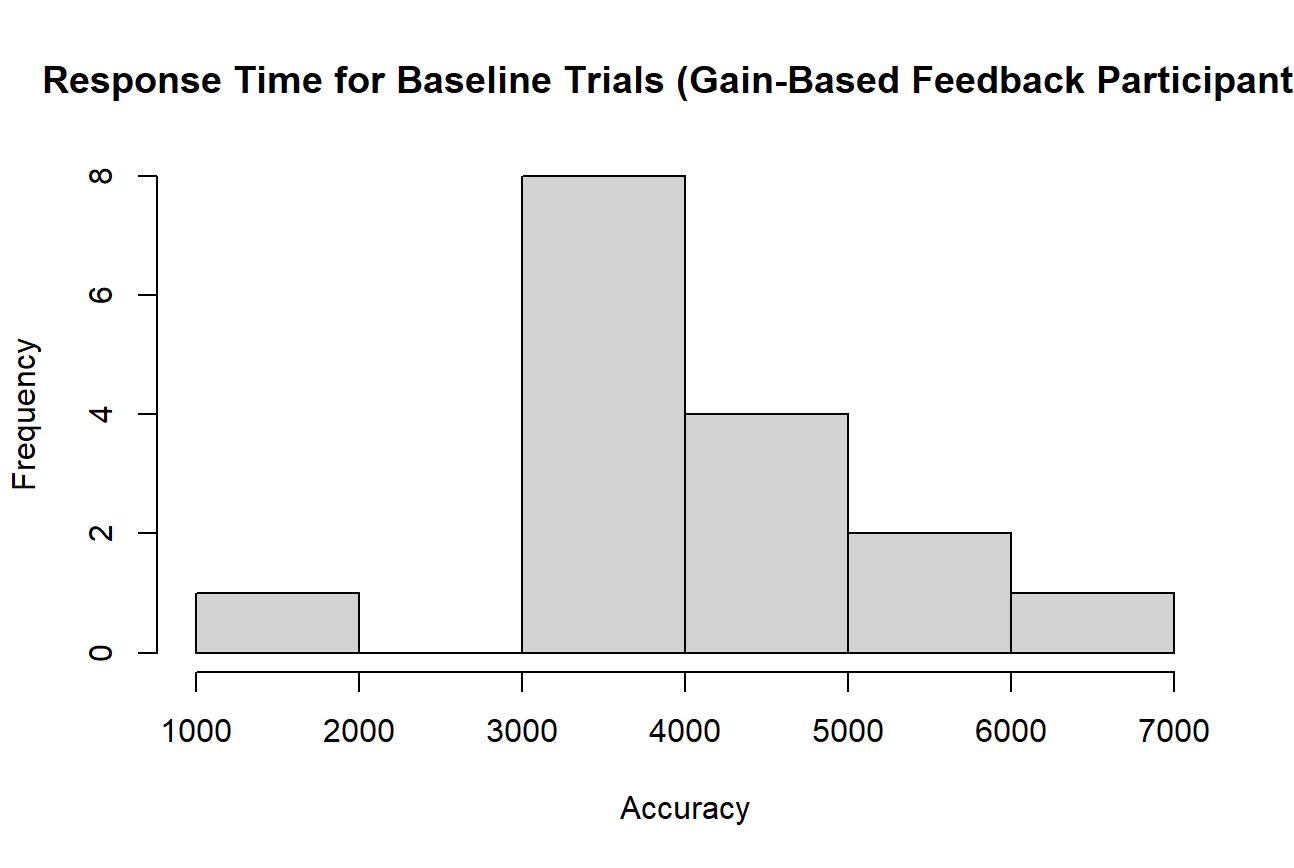
\includegraphics[width=0.8\linewidth]{images/Histograms/Response Time for Baseline Trials (Gain-Based Feedback Participants).png}
\end{figure}
\begin{figure}[H]
	\centering
	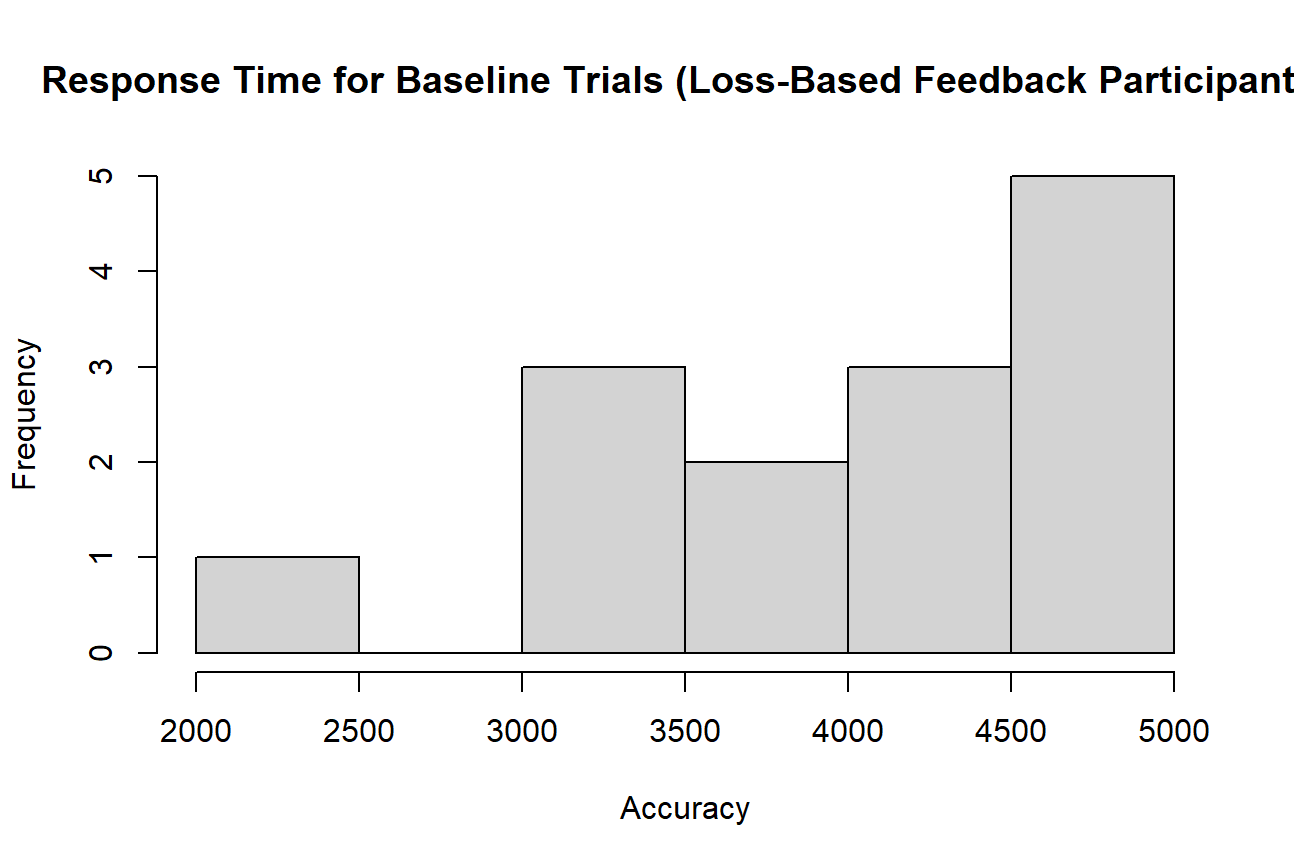
\includegraphics[width=0.8\linewidth]{images/Histograms/Response Time for Baseline Trials (Loss-Based Feedback Participants).png}
\end{figure}
\begin{figure}[H]
	\centering
	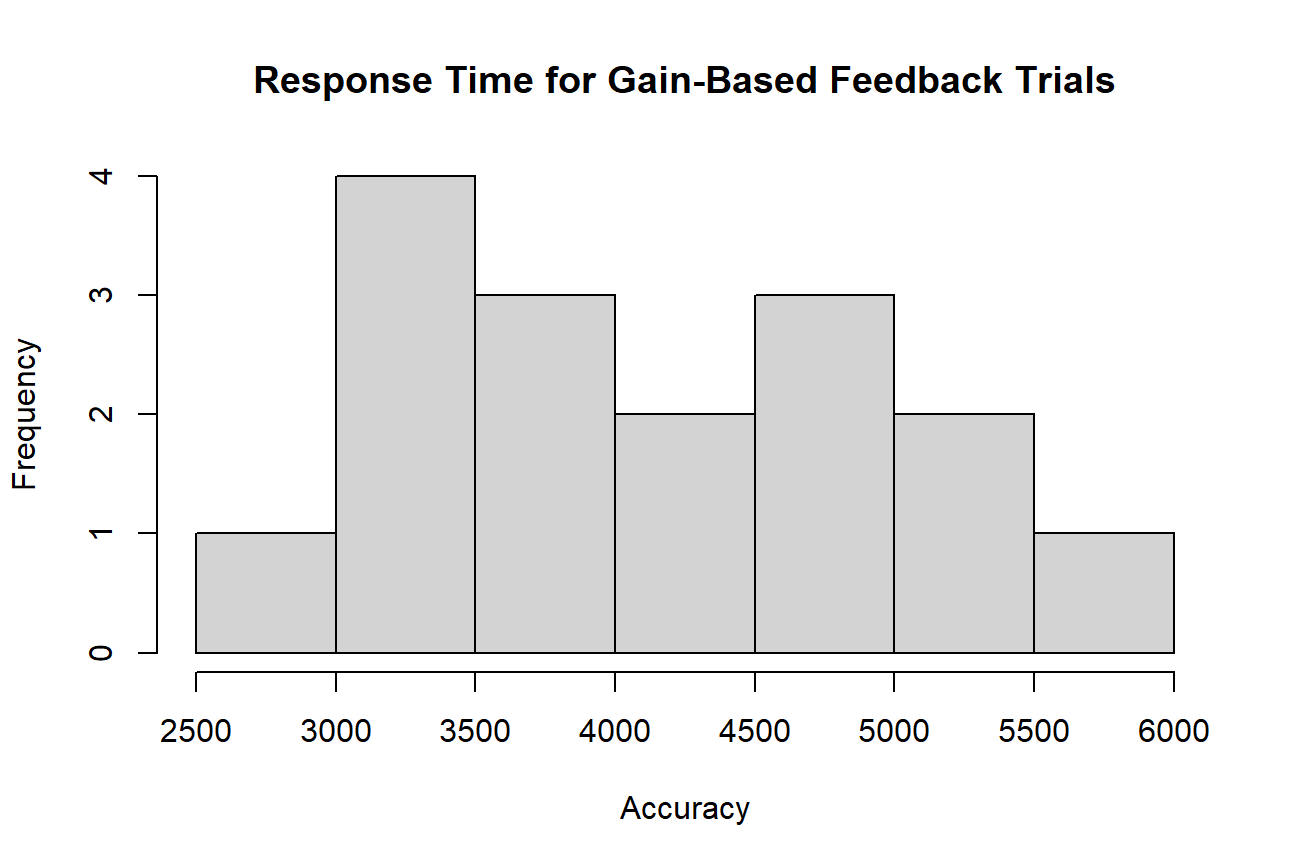
\includegraphics[width=0.8\linewidth]{images/Histograms/Response Time for Gain-Based Feedback Trials.png}
\end{figure}
\begin{figure}[H]
	\centering
	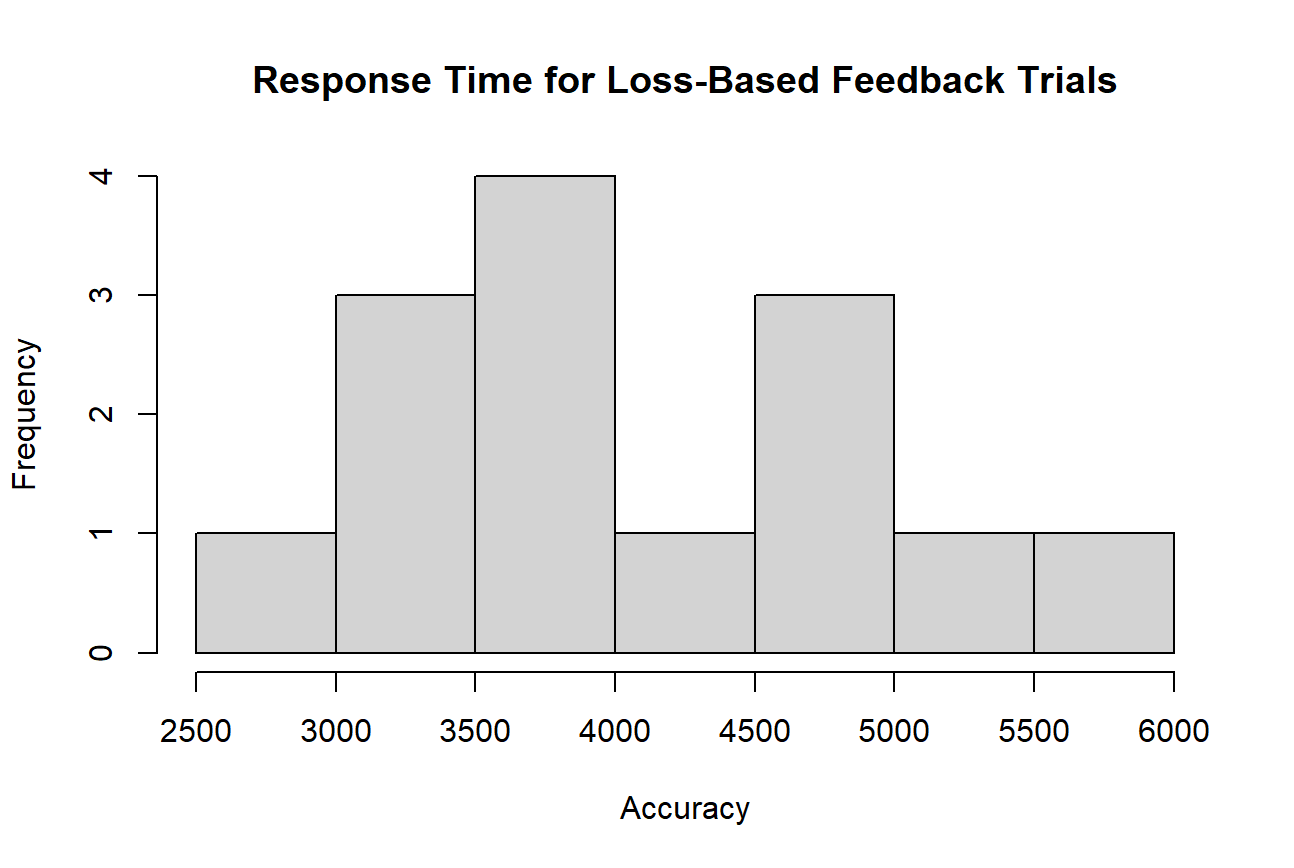
\includegraphics[width=0.8\linewidth]{images/Histograms/Response Time for Loss-Based Feedback Trials.png}
\end{figure}
\newpage
\section{Participant Comments After Finishing Feedback and Baseline Problem Sets}
\label{appdx:comments}
Comments where the participant compared the feedback and baseline problem sets are highlighted. Many found the feedback set harder, and one found it easier.
\begin{figure}[H]
    \centering
    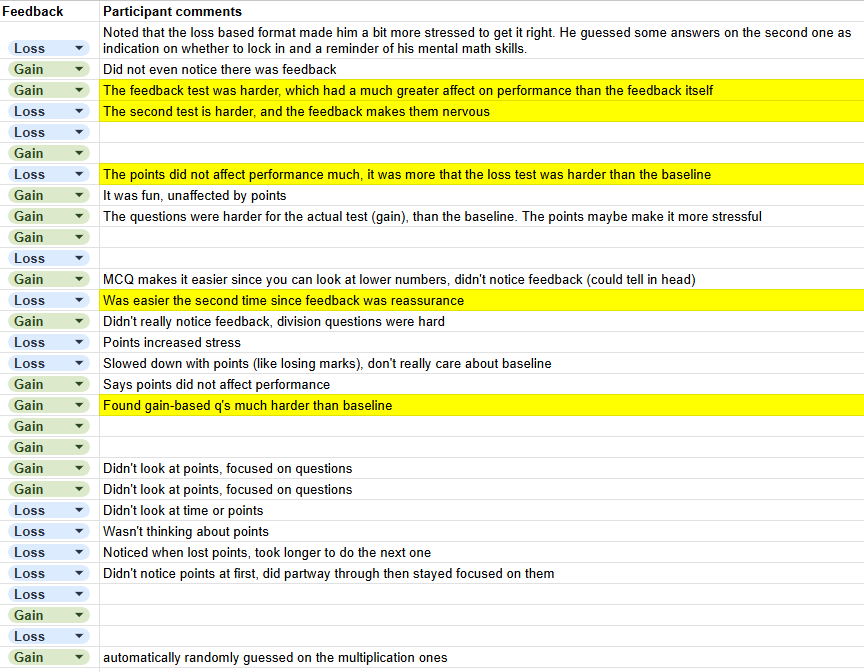
\includegraphics[width=1\linewidth]{images/participant comments after trials.png}
    \label{fig:placeholder}
\end{figure}


\end{document}